% Overleaf main document: cas-dc-template.tex
% Compiler: pdfLaTeX. Bibliography: BibTeX with cas-refs.bib.
% All manuscript text, equations, tables and captions are in this file.
% All Figure_*.pdf files are in this same directory.
% Clinical figure panels are optimized at 300 dpi; vector diagrams stay vector.
% Introduction is verbatim; abstract changes only the two author-approved DSLR values.
% New controlled analyses are identified by their own configurations.
\documentclass[a4paper,fleqn]{cas-dc}
\usepackage[authoryear]{natbib}
\usepackage[utf8]{inputenc}
\usepackage{caption}
\usepackage{tabularx}
% Use text email labels, avoiding the template thumbnail-image dependency.
\ExplSyntaxOn
\bool_gset_true:N \g_stm_nologo_bool
\ExplSyntaxOff
\ifdefined\pdfminorversion\pdfminorversion=7\fi
\usepackage{placeins}
\hypersetup{colorlinks=true,linkcolor=black,citecolor=black,urlcolor=blue,
  pdftitle={DENT-STRIDE: Domain-Configured Structured FDI Tooth Detection Across Panoramic Radiographs and Intraoral Photographs},
  pdfauthor={Jiehui Sun, Xi Wu, Ruixin Tang, Pei Wu, Shiquan Min, Jiangping Zhu, Ruijie Huang}}
\captionsetup{font=small,labelfont=bf,skip=5pt}
\setlength{\emergencystretch}{1.5em}
\newcolumntype{Y}{>{\raggedright\arraybackslash}X}
\renewcommand{\topfraction}{0.95}
\renewcommand{\bottomfraction}{0.90}
\renewcommand{\textfraction}{0.05}
\renewcommand{\floatpagefraction}{0.85}
\renewcommand{\dbltopfraction}{0.95}
\renewcommand{\dblfloatpagefraction}{0.85}

\makeatletter
\setlength{\@fptop}{0pt}
\setlength{\@dblfptop}{0pt}
\makeatother

\begin{document}
\let\WriteBookmarks\relax
\shorttitle{DENT-STRIDE: Structured FDI tooth detection}
\shortauthors{J. Sun, X. Wu et al.}
\title[mode=title]{DENT-STRIDE: Domain-Configured Structured FDI Tooth Detection Across Panoramic Radiographs and Intraoral Photographs}

% frontmatter
\author[1]{Jiehui Sun}\fnmark[1]
\author[2]{Xi Wu}\fnmark[1]
\author[1]{Ruixin Tang}
\author[1]{Pei Wu}
\author[2]{Shiquan Min}
\author[2,3]{Jiangping Zhu}[orcid=0000-0002-9756-5264]
\cormark[1]
\ead{zjp16@scu.edu.cn}
\author[1,4]{Ruijie Huang}[orcid=0000-0003-3211-518X]
\cormark[1]
\ead{ruijmhuang@gmail.com}

\affiliation[1]{organization={West China Hospital of Stomatology, Sichuan University},
 city={Chengdu},state={Sichuan},postcode={610041},country={China}}
\affiliation[2]{organization={College of Computer Science, Sichuan University},
 city={Chengdu},postcode={610065},country={China}}
\affiliation[3]{organization={National Key Laboratory of Fundamental Science on Synthetic Vision, Sichuan University},
 city={Chengdu},postcode={610065},country={China}}
\affiliation[4]{organization={Chengdu Mountain Cyan Technology Company},
 city={Chengdu},state={Sichuan},postcode={610218},country={China}}
\fntext[1]{Jiehui Sun and Xi Wu contributed equally to this work.}
\cortext[1]{Corresponding authors: Jiangping Zhu and Ruijie Huang.}


\begin{abstract}
Automatic tooth detection using the F\'ed\'eration Dentaire Internationale (FDI) numbering system provides individual tooth identification for dental assessment and structured clinical records.
Although recent detectors have improved tooth localization, variations in image acquisition, similarities in tooth appearance, and image degradation caused by blur and acquisition artifacts continue to challenge reliable FDI identity assignment.
We propose DENT-STRIDE, a framework that accounts for acquisition characteristics to achieve structured FDI tooth detection across radiographic and photographic images.
Separate prediction heads for quadrant, tooth position, and dentition type provide explicit supervision of tooth identity, complemented by prototype learning employed exclusively during training.
An independent anatomical prior adjusts classification scores using statistics of tooth center locations and bounding box shapes derived from training data, without modifying the predicted boxes.
Feature exchange across multiple scales and local contextual refinement are adapted to each acquisition domain within a shared query based detector built on DEIM and D-FINE.
We evaluate the proposed framework on DENTEX2023 panoramic radiographs containing 32 permanent tooth classes and intraoral photographs acquired using smartphones and digital single lens reflex (DSLR) cameras, covering 52 classes of permanent and primary teeth.
Averaged across three training seeds, the COCO AP values evaluated using FDI tooth labels reach 54.21, 55.46, and 73.22 for the panoramic, smartphone, and DSLR cohorts, respectively.
At a fixed confidence threshold, the corresponding F1 scores are 89.35\%, 80.73\%, and 92.84\%, respectively.
\end{abstract}
\begin{keywords}
tooth detection \sep FDI numbering \sep structured prediction \sep panoramic radiography \sep intraoral photography \sep transformer detector \sep domain shift
\end{keywords}
\maketitle


% introduction
\section{Introduction}
\label{sec:introduction}

Automatic tooth detection and identification link imaging findings to individual teeth and support structured dental records \citep{schwendicke2020artificial,sadr2024tooth}. The F\'ed\'eration Dentaire Internationale (FDI) notation encodes quadrant, tooth position, and dentition. A useful detector must therefore locate each visible tooth and assign its correct FDI label despite variable image quality and incomplete views.

Early deep learning approaches used convolutional neural networks (CNNs) to extract tooth appearance features and combined detection with additional numbering procedures. In 2019, \citet{tuzoff2019tooth} used Faster R-CNN to localize teeth in panoramic radiographs, followed by VGG-16 recognition and spatial heuristics for numbering. In 2021, \citet{bilgir2021automatic} developed a pipeline based on Faster R-CNN with Inception v2, incorporating separate models for anterior and posterior teeth and information about the jaw to support FDI assignment. These studies established the value of learned visual features for tooth recognition and showed that spatial context can complement individual tooth appearance. However, their numbering procedures were developed for panoramic radiographs and cannot be assumed to apply unchanged to photographs with a partial view of the dentition.

In parallel, Transformers introduced new ways to model relationships across an image. DETR formulated object detection as set prediction in 2020, using learned queries and bipartite matching instead of a conventional proposal pipeline \citep{carion2020detr}. In dental imaging, \citet{almalki2023masked} evaluated SimMIM and UM-MAE pretraining for a Swin Transformer applied to panoramic tooth numbering, restoration detection, and instance segmentation. This work addressed limited annotated data by learning representations from masked images before supervised fine tuning. RT-DETR subsequently improved the efficiency of detection through a hybrid encoder and query selection \citep{zhao2024rtdetr}. D-FINE refined the distributions used for box regression, while DEIM improved matching supervision and convergence \citep{peng2025dfine,huang2025deim}. These developments provide a strong basis for joint localization and classification, but the choice of detector does not itself determine how the clinical structure of FDI labels should be represented.

More recently, selective state space models have provided an alternative route to contextual modeling. Mamba uses input dependent state updates with computational complexity that scales linearly with sequence length \citep{gu2024mamba}. In 2024, DeMambaNet combined deformable convolutions and Mamba to segment dental images with poorly defined root boundaries \citep{zou2024demambanet}, while Oral-Mamba segmented caries, calculus, and gingivitis regions in intraoral photographs \citep{liu2024oral}. Hybrid designs have also combined complementary representations. In 2025, OralSeg integrated a Swin Transformer and spatial Mamba for tooth instance segmentation in cone beam computed tomography \citep{zhou2025oralseg}. T-Mamba subsequently incorporated spatial and frequency features with gated fusion for tooth segmentation in two and three dimensions \citep{hao2026tmamba}. These studies extend the available tools for representing dental anatomy, although segmentation of teeth or lesions is a different task from detecting visible teeth and assigning their FDI identities.

For FDI detection across acquisition domains, three issues remain important. First, blur, reflections, superimposed structures, and indistinct boundaries affect the visual evidence available to a detector, as illustrated in Fig.~\ref{fig:figure1}(a). Panoramic radiographs show both dental arches, whereas smartphone and digital single lens reflex (DSLR) photographs may show only part of an arch from an oblique viewpoint. Anatomical relationships that are useful in one setting may therefore be unreliable in another. Figure~\ref{fig:figure1}(b) compares detection AP across the three cohorts, illustrating differences in performance among the evaluated methods. Second, treating FDI codes as unrelated categories does not explicitly supervise their shared quadrant, position, and dentition components. Third, matching predictions to individual teeth does not ensure that every FDI label occurs only once in the image. Visual localization, clinical identity, and numbering consistency consequently need distinct modeling and evaluation.

We propose DENT-STRIDE, a framework that configures structured FDI detection for the acquisition domain within a common DEIM and D-FINE detector. Factorized heads supervise quadrant, position within the quadrant, and dentition. A bank of learned prototypes supplies additional identity supervision during training, without contributing prototype scores at inference. Separately, SpatialShape estimates the center locations and box shapes of each tooth class from training annotations and uses these fixed anatomical scores to adjust panoramic predictions. CMFA exchanges information between feature scales in the photographic configurations, and HOOA refines local, contextual, and edge responses in the Mobile configuration. These components form DENT-STRIDE-Pano, DENT-STRIDE-Mobile, and DENT-STRIDE-DSLR, with the active paths fixed for each acquisition domain rather than chosen separately for each image.

The main contributions are threefold:
\begin{enumerate}
    \item We introduce explicit FDI identity supervision through factorized clinical labels and a learned prototype bank, distinguishing auxiliary training objectives from the factor score correction used at inference in the Mobile configuration.
    \item We define an anatomical scoring model using tooth center and box shape statistics derived from training annotations. This prior is separate from learned identity prototypes, and its effects are evaluated with fixed detector weights.
    \item We establish a common detection framework with configurations for panoramic, smartphone, and DSLR images, and evaluate it through experiments with multiple training seeds, retrained component ablations, and separate measures of localization, FDI identity, and numbering consistency.
\end{enumerate}

% figure01
\begin{figure*}[t]
\centering
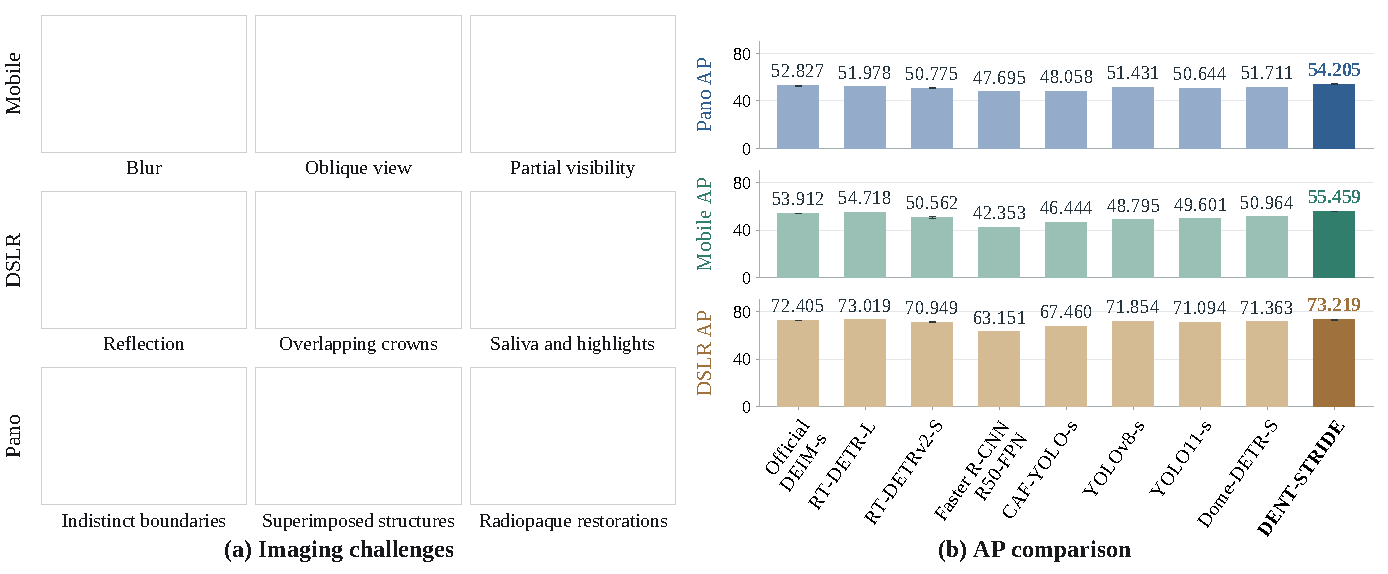
\includegraphics[width=\textwidth]{Figure_1.pdf}
\caption{Imaging challenges and detection performance across three dental image cohorts. (a) Representative smartphone (Mobile), DSLR, and panoramic (Pano) image regions illustrate blur, oblique views, partial visibility, reflections, overlapping crowns, saliva, indistinct boundaries, superimposed structures, and radiopaque restorations. All image tiles have the same size and a 3:2 aspect ratio. (b) COCO AP, expressed in percentage points, for nine detectors on the three validation cohorts. The vertical bar charts share the same model order and a scale from 0 to 90 AP. Blue, teal, and ochre represent Pano, Mobile, and DSLR, respectively; darker shades highlight DENT-STRIDE. Bar labels give the reported AP. Error bars indicate standard deviation of the three reported runs; DENT-STRIDE Pano and Mobile use the selected three of five completed seeds. Single-run results have no error bars.}
\label{fig:figure1}
\end{figure*}

% related work
\section{Related work}
\label{sec:related-work}

\subsection{Tooth localization and numbering across acquisition settings}

Learning-based tooth identification can be organized into localization followed by recognition, joint detection and enumeration, and segmentation-based identification. In panoramic radiography, \citet{tuzoff2019tooth} combined Faster R-CNN localization with VGG-16 tooth recognition and spatial-arrangement heuristics. \citet{muramatsu2021tooth} classified detected teeth by tooth type and restoration condition, using differently sized image inputs to incorporate contextual information. These studies illustrate the complementary roles of local tooth appearance and surrounding anatomy, while their outputs and evaluation endpoints differ from a single FDI-aware detection task.

Joint dental analysis extends enumeration to associated findings. DENTECT couples quadrant processing, tooth enumeration, and treatment detection in panoramic images \citep{yuksel2021dentect}, while DENTEX provides hierarchical quadrant, enumeration, and diagnostic annotations for benchmarking abnormal-tooth detection \citep{hamamci2023dentex}. Photographic analysis is a related but distinct setting: \citet{yoon2024caries} integrated tooth-number recognition and caries detection in intraoral photographs. Bitewing segmentation and numbering further demonstrate that visible-field coverage is task-specific \citep{tekin2022bitewing}, rather than interchangeable with panoramic or photographic whole-image evaluation. Primary/permanent tooth numbering in digital impressions \citep{vannistelrooij2025teeth} and tooth instance segmentation in CBCT \citep{zhou2025oralseg} further illustrate the diversity of acquisition dimensionality and annotation scope.

These studies establish tooth recognition across several imaging settings, but their imaging geometries, label inventories, annotation targets, and matching criteria differ. A permanent-tooth radiographic task and a mixed-dentition photographic task impose different identity requirements, while photographic viewpoints alter the spatial relationships that are visible within an image. This motivates a framework that makes acquisition-specific feature processing and identity supervision explicit while retaining a common detection formulation. DENT-STRIDE follows this design: its configurations share the query detector, but distinguish the identity and geometric information appropriate to each acquisition setting.

\subsection{Hierarchical identity learning and prototype supervision}

Tooth identity can be predicted as a flat category or decomposed into clinically meaningful attributes. \citet{zhang2018labeltree} used a label tree and cascaded convolutional networks to divide recognition of 32 tooth positions in periapical radiographs into subproblems. DENTEX similarly makes quadrant and enumeration explicit in its annotation hierarchy \citep{hamamci2023dentex}. Such decompositions expose the structure of the label space, but a cascade operating on image regions and auxiliary targets attached to a shared detection query represent different computational choices.

Representation-based supervision offers a complementary route. Prototypical networks classify embeddings through distances to class representatives computed from support examples \citep{snell2017prototypical}. This provides a useful reference for class-centered representation learning, but does not make every prototype-based auxiliary branch a few-shot classifier. In DENT-STRIDE, multiple learnable, normalized representatives per FDI class supervise matched decoder queries through cosine similarity; they are not support-set averages, spatial templates, or a replacement for the detection head.

For query-based dental detection, the relevant distinction is between learning an identity representation and changing the scores used for detection. DENT-STRIDE separates factor-target supervision, a bounded factor-score correction where enabled, and training-only prototype supervision. Quadrant, within-quadrant position, and dentition targets are derived from the clinical FDI map; because quadrant already contains dentition information, they are structured decompositions rather than independent anatomical variables. Attaching these targets to shared decoder queries avoids a separate region-recognition cascade and allows identity supervision to be examined independently of geometric class-score correction.

\subsection{Anatomical scoring and dental-chart consistency}

Anatomical information may enter a dental system through learned features, explicit ordering rules, or geometric post-processing. The spatial heuristics used by \citet{tuzoff2019tooth} refine tooth recognition according to dental arrangement. \citet{ali2023teeth} combined separate tooth and prosthesis detectors with a priori optimization, incorporating complete restorations into enumeration under the universal numbering system. Their formulation illustrates the importance of treatment-dependent anatomy, but its restoration-aware assignment should not be conflated with FDI classification or with a class-conditional box prior.

Class-conditional box scoring offers a different way to incorporate anatomy. SpatialShape uses normalized tooth centers and joint log-width/log-height statistics from the training annotations to define fixed scores for each FDI class. Unlike a learned appearance representation, these statistics describe where a class occurs and how its box is shaped within the acquisition field. The scores adjust class ranking without moving the predicted boxes or replacing the detection head. Separating center and shape contributions also makes it possible to examine which aspect of the geometric information influences the output.

Geometric plausibility also differs from complete chart consistency. Accurate localization and identity among matched teeth do not, by themselves, require each visible FDI code to occur only once. A class-score adjustment without a uniqueness or assignment constraint cannot guarantee that property. We therefore distinguish detector AP, localization coverage, matched-tooth FDI accuracy, and repeated-label diagnostics. These endpoints describe different aspects of the output rather than substitutes for a clinically validated charting pipeline.

\subsection{Query detection and multiscale feature refinement}

General object detectors provide complementary design choices for dental localization. Faster R-CNN uses region proposals and region-wise prediction \citep{ren2015faster}, whereas DETR treats detection as set prediction through learned queries and bipartite matching, without an added non-maximum suppression stage \citep{carion2020detr}. RT-DETR develops an efficient hybrid encoder and query selection for real-time set prediction \citep{zhao2024rtdetr}; RT-DETRv2 further refines its training and deployment design \citep{lv2024rtdetrv2}. These alternatives motivate complete-system comparisons, with pretraining and native optimization differences reported rather than assumed absent.

Within this family, D-FINE refines bounding-box probability distributions and transfers localization knowledge across decoder layers \citep{peng2025dfine}. DEIM addresses convergence through denser one-to-one supervision and Matchability-Aware Loss \citep{huang2025deim}. DENT-STRIDE adopts their detection scaffold instead of presenting matching or distribution refinement as new contributions. Its dental-specific additions act on the representations and identities of tooth queries, or on class scores after decoding; detection matching does not impose a unique clinical tooth label across all retained query--class pairs.

Multiscale representation and feature selection operate at another level. Feature Pyramid Networks propagate semantic information through top-down and lateral connections \citep{lin2017fpn}, while CBAM uses channel and spatial attention to refine convolutional features \citep{woo2018cbam}. These mechanisms address feature scale and relevance, rather than the clinical relationships between FDI labels. CMFA applies reciprocal channel-gated exchange to aligned adjacent-scale features before spatial modulation. HOOA instead combines local, dilated-context, high-pass, and multiplicative responses within a feature level, followed by joint gating and a residual update with a bounded scaling coefficient. This separation permits cross-scale exchange and within-scale refinement to be evaluated as distinct operations alongside structured tooth-identity supervision.



% methods
\section{Methods}
\label{sec:methods}

\subsection{Overview of DENT-STRIDE}
\label{sec:overview}

DENT-STRIDE separates multiscale visual processing, query-level identity learning, and anatomical score correction within an acquisition-configured detector (Fig.~\ref{fig:figure2}). The shared scaffold comprises an HGNetv2-B0 backbone, three 256-channel projected feature levels, a hybrid encoder, and a three-layer D-FINE decoder with 300 ordinary queries. DEIM supplies matching and detection losses \citep{huang2025deim,peng2025dfine}. The configuration is fixed for each acquisition domain before inference.


% figure02
\begin{figure*}[tp]
\centering
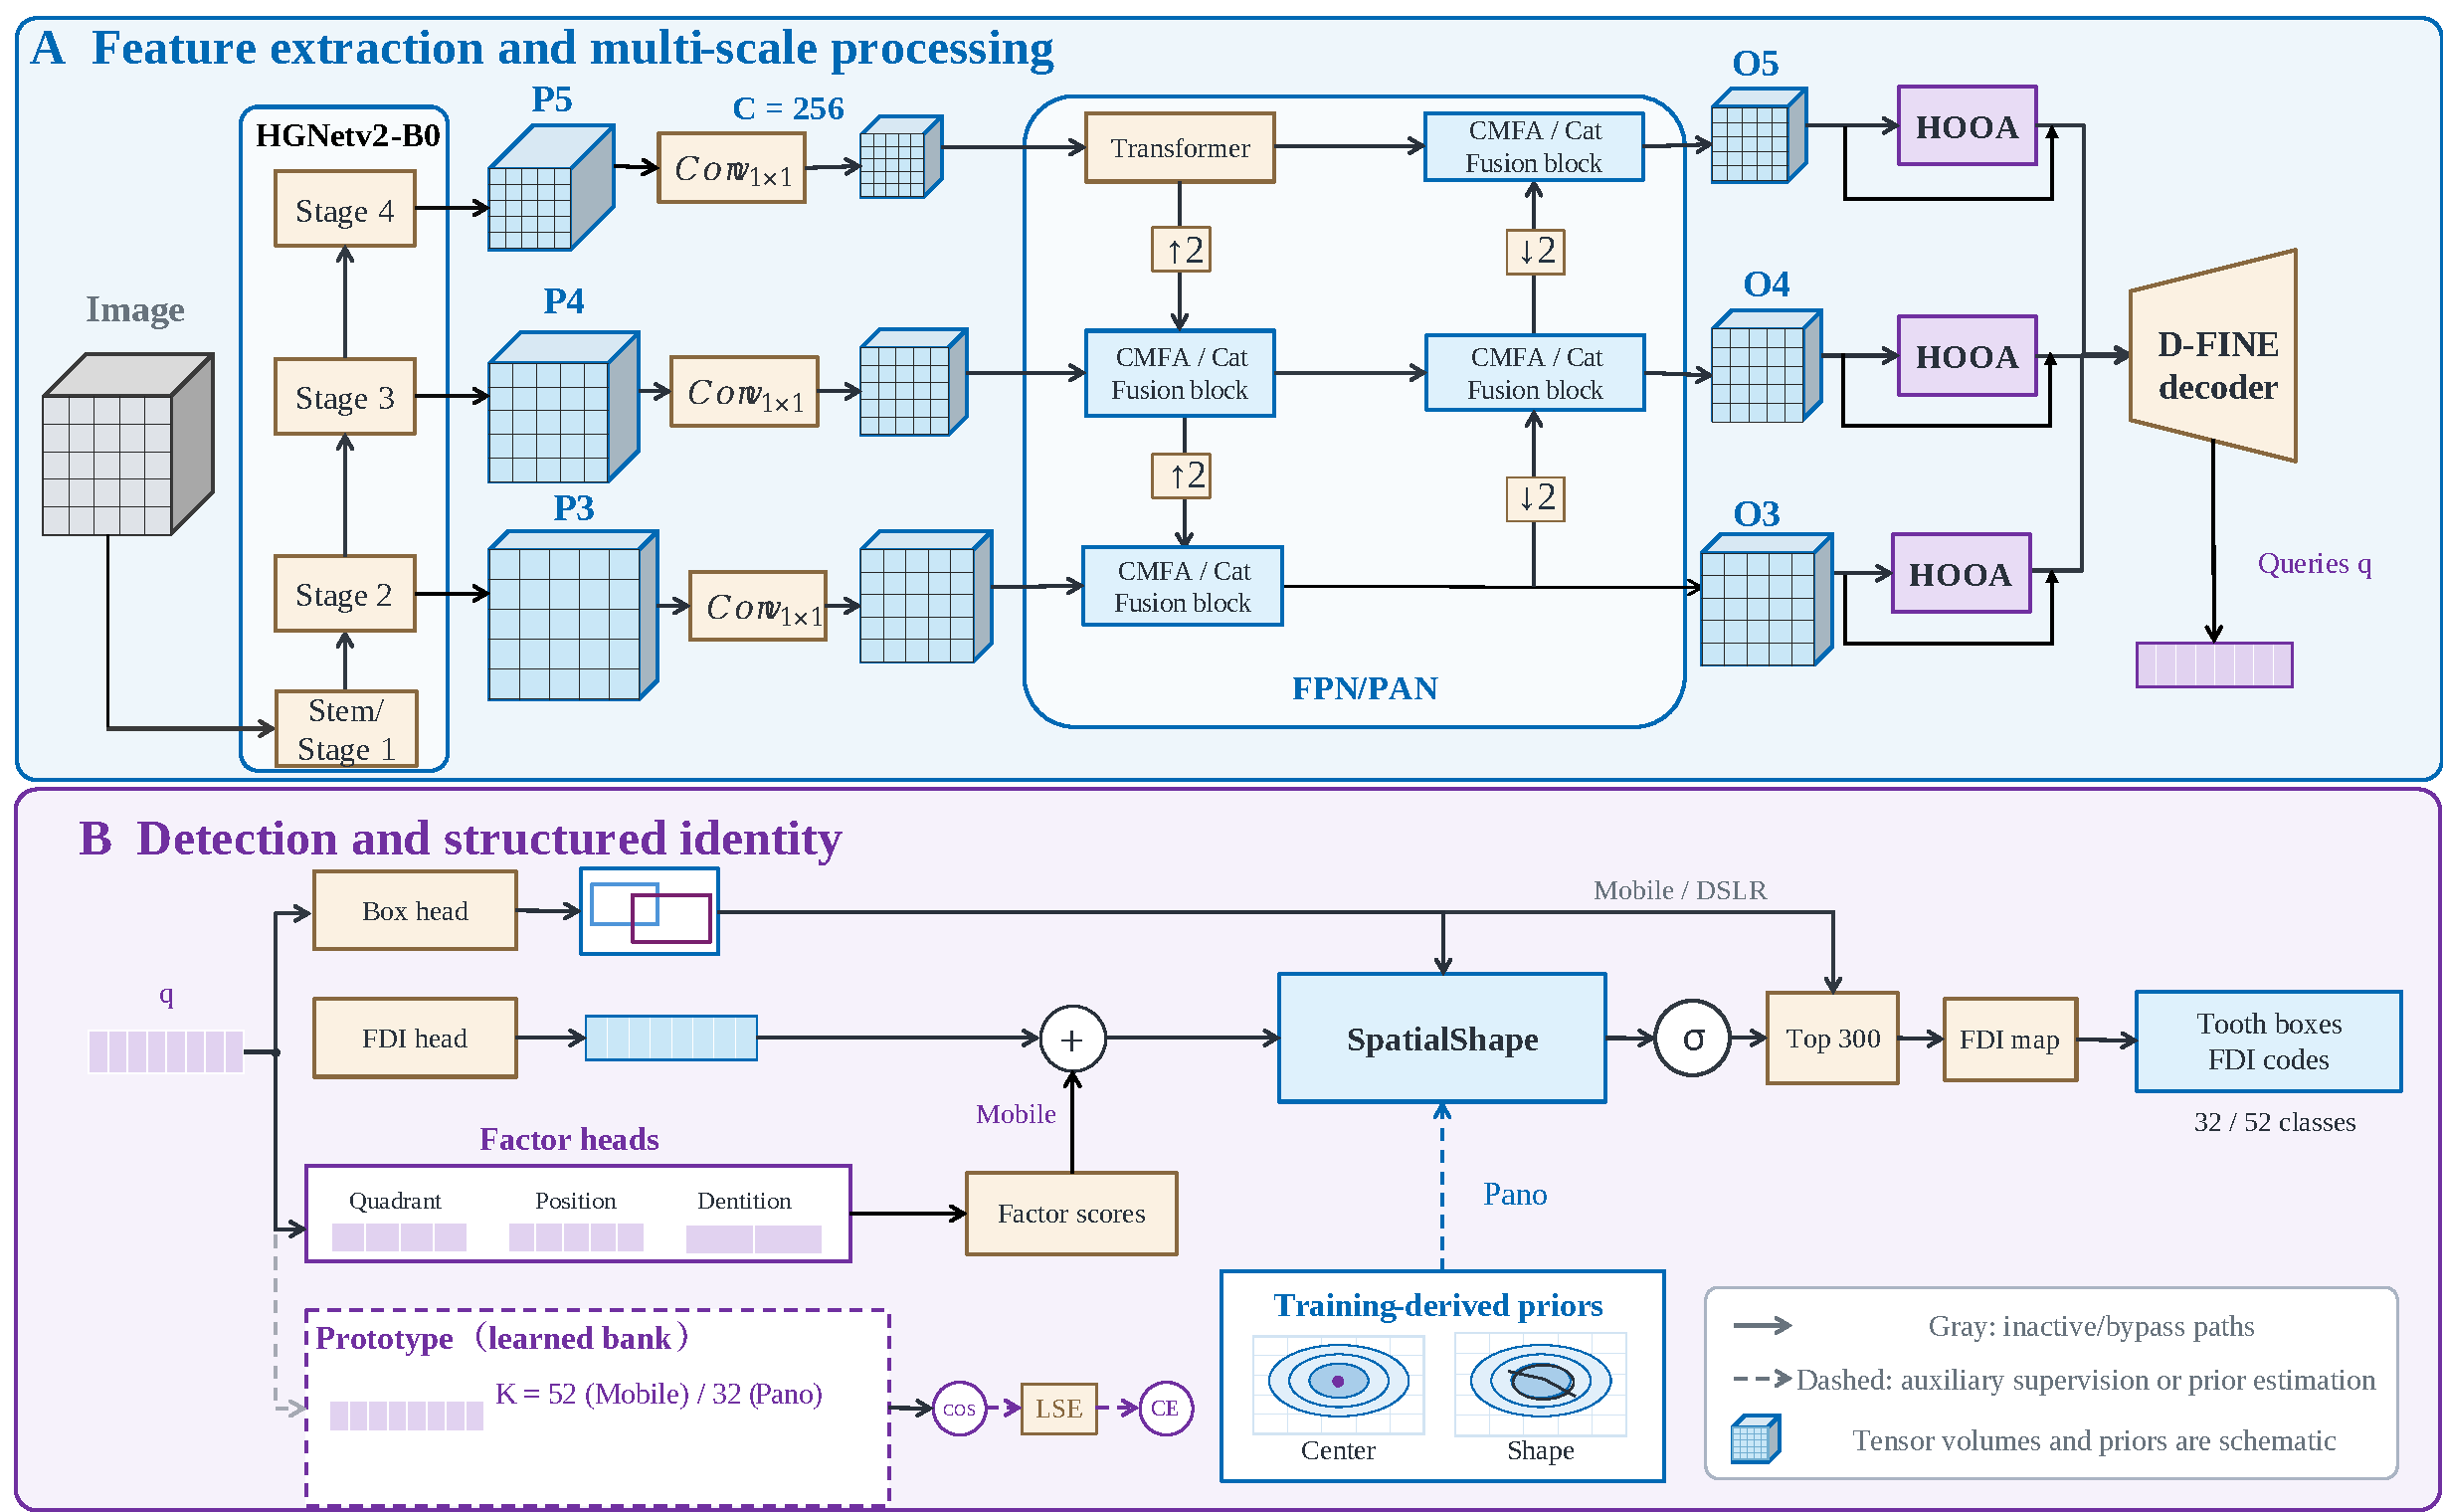
\includegraphics[width=\textwidth]{Figure_2.pdf}
\caption{Acquisition-configured DENT-STRIDE architecture. (A) HGNetv2-B0 features at strides 8, 16, and 32 are projected to 256 channels. The highest-stride transformer precedes top-down FPN and bottom-up PAN aggregation. Four fusion sites use CMFA in Mobile and DSLR, and concatenation in Pano; the base fusion blocks restore 256 channels. HOOA refines the three output levels in Mobile. (B) Decoder queries supply box and FDI heads and structured identity supervision. The learned bank contains four prototypes per class (K = 52 in Mobile and 32 in Pano), with a shared prototype temperature of $\tau$ = 0.50 in both configurations. Prototype scores provide training-only auxiliary supervision; factor-logit correction is enabled only in Mobile. The Pano SpatialShape prior modifies candidate logits before sigmoid scoring and top-300 selection. Cohort-specific label maps decode predictions to clinical FDI codes. The DSLR configuration applies additional parameter-rank decay during training, without initialization rollback. Gray paths bypass inactive modules; dashed paths denote auxiliary supervision or training-derived prior estimation. Tensor volumes and prior glyphs are schematic.}
\label{fig:figure2}
\end{figure*}



The backbone produces features at strides 8, 16, and 32. After projection, the coarsest level is processed by a transformer, followed by top-down feature pyramid network (FPN) and bottom-up path aggregation network (PAN) operations. Cross-scale mutual feature aggregation (CMFA) operates at four adjacent-scale fusion sites for the Mobile and DSLR configurations; high-order omni-attention (HOOA) refines the three output levels only for Mobile. The decoder produces query representations for box regression and FDI classification. Factor and prototype supervision are attached to the same queries, while their prediction-time roles are distinct: Mobile uses a small factor-score correction, prototypes supply training supervision only, and Pano uses fixed geometry scores before final query--class selection. The cohort label map converts class indices into clinical FDI codes.

The configurations are DENT-STRIDE-Pano (Factor + Prototype with SpatialShape), DENT-STRIDE-Mobile (CMFA + HOOA with Factor + Prototype), and DENT-STRIDE-DSLR (CMFA with additional rank-dependent decay). Pano uses factor/prototype auxiliary supervision without factor-score fusion; Mobile uses both auxiliary supervision and factor-score fusion; DSLR uses no identity auxiliary branches or initialization rollback. The training and inference roles are defined below; acquisition-specific settings are summarized in Section~\ref{sec:implementation}.

\subsection{Structured identity learning}
\label{sec:identity}

\subsubsection{Factorized FDI supervision and score fusion}
\label{sec:factors}

Let $z_{ik}$ denote the FDI logit of query $i$ for class $k$ before factor fusion, and let $\mathbf{a}_{i}^{(h)}$ be the logits of factor head $h\in\{q,p,d\}$ (quadrant, within-quadrant position, and dentition). The three heads have 8, 8, and 2 outputs, respectively. The dataset label map converts class $k$ to its clinical FDI code $f_k$ and hence to zero-based factor indices $q(k)=\lfloor f_k/10\rfloor-1$, $p(k)=(f_k\bmod 10)-1$, and $d(k)=0$ for primary teeth or $1$ for permanent teeth. With $\boldsymbol{\ell}_{i}^{(h)}=\operatorname{logsoftmax}(\mathbf{a}_{i}^{(h)})$, the mapped factor scores are first combined:
\begin{equation}
 u_{ik}=\alpha_q\ell_{i,q(k)}^{(q)}
       +\alpha_p\ell_{i,p(k)}^{(p)}
       +\alpha_d\ell_{i,d(k)}^{(d)}.
 \label{eq:factor-score}
\end{equation}
The combined score is then centered over the $K$ FDI classes and clipped once:
\begin{equation}
 \widetilde z_{ik}=z_{ik}
 +\operatorname{clip}\!\left(u_{ik}-\max_{1\leq j\leq K}u_{ij},-6,0\right).
 \label{eq:factor-fusion}
\end{equation}
For DENT-STRIDE-Mobile, the fusion weights are $\alpha_q=0.10$, $\alpha_p=0.05$, and $\alpha_d=0.03$. Thus, weighting precedes centering and clipping; the three factor branches are not clipped separately. The correction is applied to ordinary detection queries at each evaluated decoder layer during training and inference, excluding denoising queries during training. The native D-FINE localization-quality adjustment follows this operation. DENT-STRIDE-Pano uses the factor heads for auxiliary supervision without this inference correction. Factor targets are supervised by mean cross-entropy over matched queries, with quadrant/position/dentition weights $(0.08,0.08,0.03)$ for Mobile and $(0.10,0.10,0.05)$ for Pano. The same head-specific weights apply to intermediate-decoder and denoising outputs when those factor logits are present.

Quadrant outputs cover permanent and primary quadrants, so dentition is an additional supervised decomposition rather than an independent clinical variable. All factors are decoded through the clinical label map.

\subsubsection{Prototype auxiliary supervision}
\label{sec:prototypes}

Let $\mathbf h_i\in\mathbb R^{256}$ be the final-decoder representation of an ordinary query, and let $\mathbf P_{kr}\in\mathbb R^{256}$ be learnable prototype $r\in\{1,2,3,4\}$ for FDI class $k$. Each prototype coordinate is initialized independently from a zero-mean Gaussian with standard deviation $0.02$. Queries and prototypes are normalized along the feature dimension:
\begin{equation}
 \begin{aligned}
 \widehat{\mathbf h}_i
  &=\frac{\mathbf h_i}{\max(\lVert\mathbf h_i\rVert_2,\varepsilon)},\\
 \widehat{\mathbf P}_{kr}
  &=\frac{\mathbf P_{kr}}{\max(\lVert\mathbf P_{kr}\rVert_2,\varepsilon)},
 \qquad \varepsilon=10^{-12}.
 \end{aligned}
 \label{eq:prototype-normalization}
\end{equation}
Cosine similarities are divided by temperature $\tau$ and aggregated across the four prototypes using LogSumExp:
\begin{equation}
 \begin{aligned}
 t_{ikr}&=\widehat{\mathbf h}_i^{\mathsf T}\widehat{\mathbf P}_{kr},\\
 r_{ik}&=\log\left[\sum_{r=1}^{4}\exp(t_{ikr}/\tau)\right].
 \end{aligned}
 \label{eq:prototype-score}
\end{equation}
For the final-output one-to-one matching set $\mathcal M$ containing $N$ matched queries, with matched target class $y_i$, the weighted prototype loss is
\begin{equation}
 \mathcal L_{\mathrm{proto}}
 =-\frac{\lambda_{\mathrm{proto}}}{N}
  \sum_{i\in\mathcal M}\log
  \frac{\exp(r_{i,y_i})}{\sum_{k=1}^{K}\exp(r_{ik})}.
 \label{eq:prototype-loss}
\end{equation}
Both identity configurations use four prototypes per class with a shared temperature of $\tau=0.50$. The prototype-loss weights are $0.03$ for Mobile and $0.05$ for Pano. The loss averages over matched final-layer ordinary queries and is zero for an empty match set. Queries and prototypes both receive gradients, but prototype scores do not alter inference logits. Unsupported smartphone classes 18, 28, 38, and 48 are excluded from prototype interpretation. The Mobile component ablations described in Section~\ref{sec:component-ablations} use a fixed prototype temperature of $\tau=0.50$.

\subsection{Training-derived SpatialShape prior}
\label{sec:spatialshape}

Templates are estimated from the 16,234 valid training boxes in the 570 DENTEX2023 training images, separately for the 32 permanent FDI classes. For a box $(x,y,w,h)$ in an image of width $W$ and height $H$, define normalized center and log-shape features:
\begin{equation}
 \begin{aligned}
 \mathbf c&=\left(\frac{x+w/2}{W},\frac{y+h/2}{H}\right)^{\mathsf T},\\
 \mathbf s&=\begin{pmatrix}
  \log\max(w/W,10^{-5})\\
  \log\max(h/H,10^{-5})
 \end{pmatrix}.
 \end{aligned}
 \label{eq:geometry-features}
\end{equation}
For feature type $a\in\{c,s\}$ and the $n_k$ training boxes of class $k$, the mean is $\boldsymbol\mu_k^{(a)}=n_k^{-1}\sum_{n=1}^{n_k}\mathbf a_{kn}$. Writing the centered feature as $\mathbf e_{kn}^{(a)}=\mathbf a_{kn}-\boldsymbol\mu_k^{(a)}$, the full two-dimensional sample covariance, including its off-diagonal term, is regularized as
\begin{equation}
 \boldsymbol\Sigma_k^{(a)}
 =\frac{1}{n_k-1}\sum_{n=1}^{n_k}
   \mathbf e_{kn}^{(a)}\bigl(\mathbf e_{kn}^{(a)}\bigr)^{\mathsf T}
  +10^{-3}\mathbf I_2.
 \label{eq:geometry-covariance}
\end{equation}
All 32 DENTEX classes have at least two training boxes. In the general construction, a single supported box uses covariance $10^{-3}\mathbf I_2$, and an unsupported class receives a zero template score. At inference, the predicted normalized center and log-width/log-height are scored by the corresponding class-specific quadratic forms. With $\mathbf e_{ik}^{(a)}=\mathbf a_i-\boldsymbol\mu_k^{(a)}$,
\begin{equation}
 \begin{aligned}
 g_{ik}^{(a)}=\operatorname{clip}\!\Bigl[
 &-\tfrac12\bigl(\mathbf e_{ik}^{(a)}\bigr)^{\mathsf T}
  \bigl(\boldsymbol\Sigma_k^{(a)}\bigr)^{-1}\mathbf e_{ik}^{(a)},\\[-1pt]
 &-20,0\Bigr].
 \end{aligned}
 \label{eq:geometry-score}
\end{equation}
These joint Mahalanobis scores omit log-determinants, density-normalization constants, and empirical class-frequency terms. Each score is separately centered across classes and clipped again:
\begin{equation}
 \delta_{ik}^{(a)}=\operatorname{clip}\!\left[
 g_{ik}^{(a)}-\max_{1\leq j\leq K}g_{ij}^{(a)},-6,0\right].
 \label{eq:geometry-correction}
\end{equation}
Let $z_{ik}^{\mathrm{det}}$ denote the decoder output logit before post-processing. Spatial, shape, and view terms are combined additively in logit space, followed by sigmoid:
\begin{equation}
 \begin{aligned}
 z_{ik}^{\mathrm{SS}}&=z_{ik}^{\mathrm{det}}
  +0.20\delta_{ik}^{(c)}+0.05\delta_{ik}^{(s)}+0.20v_k,\\
 \pi_{ik}&=\operatorname{sigmoid}\bigl(z_{ik}^{\mathrm{SS}}\bigr).
 \end{aligned}
 \label{eq:spatialshape-fusion}
\end{equation}
The view term $v_k$ is $0$ for an FDI class included in the specified view and $-2$ otherwise. For the DENTEX panoramic setting, all 32 permanent FDI classes are included, so $v_k=0$ for every class and the view term has no numerical effect. The two geometric contributions are therefore bounded jointly within $[-1.50,0]$. No appearance-prototype score is added. The final 300 query--class pairs are selected by descending $\pi_{ik}$, without added non-maximum suppression or an FDI-uniqueness assignment constraint; box coordinates are not changed by the prior. Means and covariance inverses are fixed training-derived statistics and are not learned from validation images. SpatialShape is used by DENT-STRIDE-Pano, not DENT-STRIDE-Mobile.

Figure~\ref{fig:figure3} visualizes the training-derived center templates. These fixed geometric statistics are distinct from the learnable identity bank. The four-way same-checkpoint comparison in Section~\ref{sec:prior-ablation} isolates center and shape scoring effects.


% figure03
\begin{figure*}[tp]
\centering
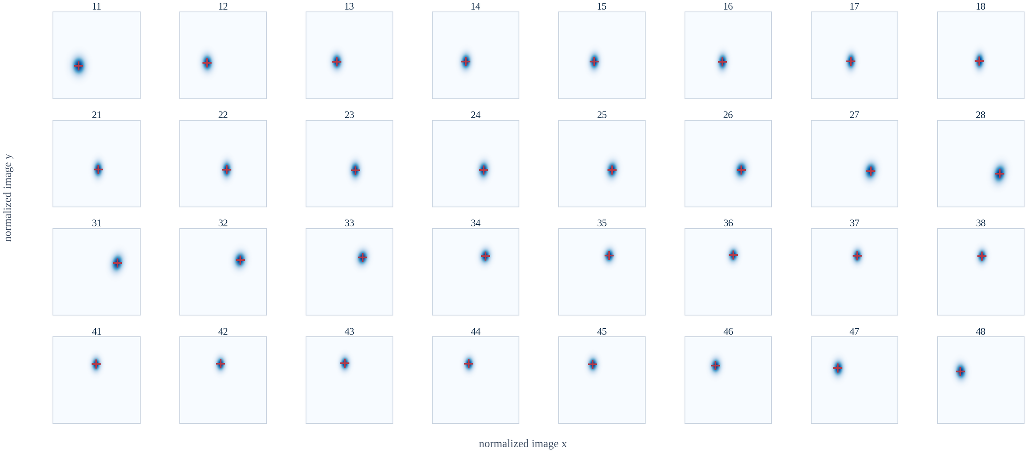
\includegraphics[width=\textwidth]{Figure_3.pdf}
\caption{Training-derived center templates for the 32 permanent DENTEX FDI classes. Each panel shows the class-specific center distribution in normalized image coordinates, based on training-box means and full regularized covariances. The templates are fixed at inference and are separate from the learnable appearance prototypes.}
\label{fig:figure3}
\end{figure*}



\subsection{Cross-scale feature aggregation and local refinement}
\label{sec:features}

\subsubsection{Cross-scale mutual feature aggregation}
\label{sec:cmfa}

CMFA replaces native concatenation at four adjacent-scale aggregation sites: two top-down FPN and two bottom-up PAN sites (Fig.~\ref{fig:figure4}). Aligned inputs $A$ and $B$ each have 256 channels. Their concatenation is globally average-pooled and passed through a $1\times1$ convolution, SiLU, a second $1\times1$ convolution, and sigmoid to obtain channel gates $g_A$ and $g_B$. The reciprocal cross-enhanced features $A'=A+g_B\odot B$ and $B'=B+g_A\odot A$ are concatenated into $Z=\operatorname{Cat}(A',B')$, where $\odot$ denotes elementwise multiplication with broadcasting. Channel-wise mean and maximum maps of $Z$ then drive a $7\times7$ convolution and sigmoid spatial gate $G_s$. The gated output $Y=Z\odot G_s$ retains 512 channels and feeds the next fusion block, which restores 256 channels. In gate ablations, the subsequent network and output dimensions are held fixed; disabling a gate removes its modulation without replacing the feature projection.


% figure04
\begin{figure*}[tp]
\centering
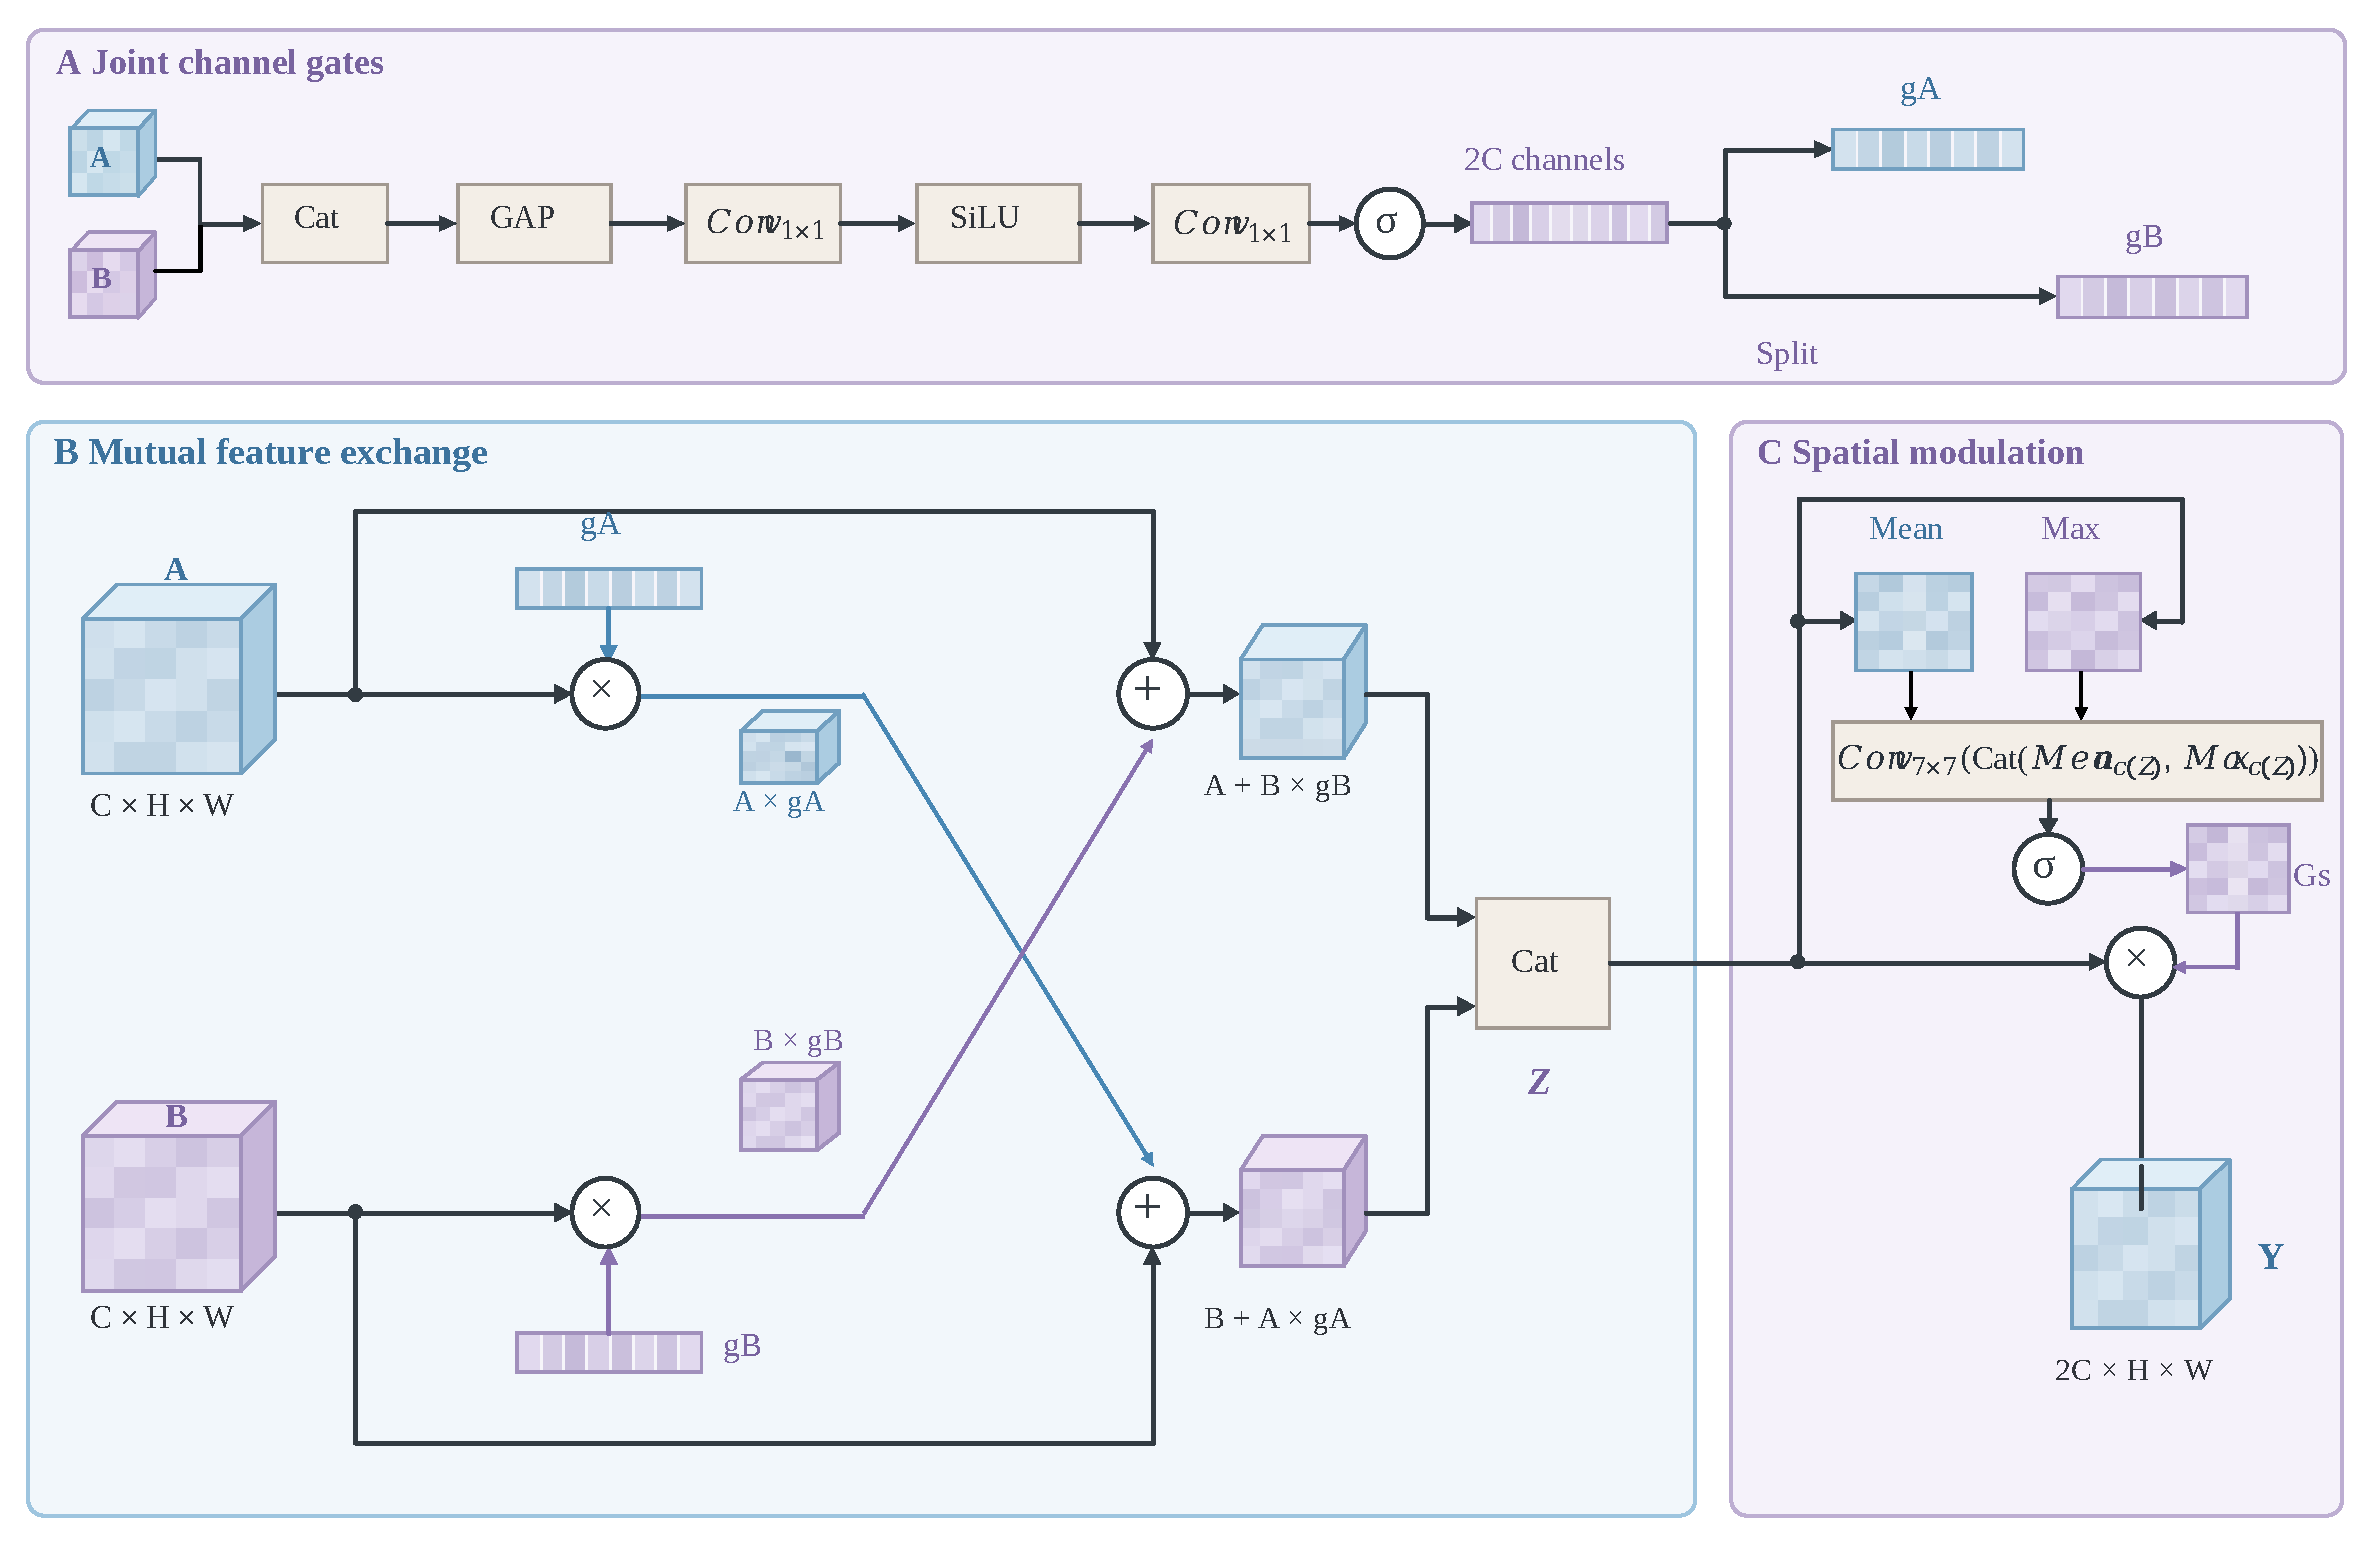
\includegraphics[width=\textwidth]{Figure_4.pdf}
\caption{Cross-scale mutual feature aggregation (CMFA). (A) Aligned C-channel features A and B jointly supply channel gates through concatenation, global-average pooling, pointwise projection, SiLU, a second projection, and sigmoid; the result is split into gA and gB. (B) Gated cross-feature exchange forms Z = Cat(A + B $\odot$ gB, B + A $\odot$ gA). (C) Channel mean and maximum of Z supply a 7$\times$7 sigmoid spatial gate Gs, giving Y = Z $\odot$ Gs. C = 256 and the output has 2C = 512 channels. Circular $\times$/+ nodes are elementwise multiplication/addition; grid colours illustrate tensor layout rather than measured activations.}
\label{fig:figure4}
\end{figure*}



\subsubsection{High-order omni-attention}
\label{sec:hooa}

Mobile uses HOOA after encoder aggregation (Fig.~\ref{fig:figure5}). Given an input feature $X$, the local branch produces $L$ using a depthwise $3\times3$ convolution followed by a pointwise $1\times1$ convolution. The context branch produces $C$ using a depthwise $7\times7$ convolution with dilation 3 followed by a pointwise convolution. The high-pass branch first computes $X-\operatorname{AvgPool}_3(X)$, then applies a depthwise $3\times3$ convolution and a pointwise convolution to obtain the edge response $E$. The multiplicative local--context response is $L\odot\operatorname{sigmoid}(C)$. These responses are concatenated and projected to a 256-channel feature:
\[
 F=\operatorname{PW}_{1\times1}\!\left(
 \operatorname{Cat}\bigl[L,L\odot\operatorname{sigmoid}(C),E\bigr]\right).
\]
The local, edge, and output projections use batch normalization and SiLU after each convolution. The context branch uses batch normalization and SiLU after its depthwise convolution and batch normalization after its pointwise convolution.

Channel and spatial gates are computed from the same pre-gated feature $F$. The channel gate uses global average pooling, pointwise projection, SiLU, a second pointwise projection, and sigmoid. The spatial gate uses the channel-wise mean and maximum of $F$, followed by a $7\times7$ convolution and sigmoid. Their product modulates the residual update,
\[
 \begin{aligned}
 Y&=X+\alpha F\odot G_c(F)\odot G_s(F),\\
 \alpha&=0.30\operatorname{sigmoid}(s),
 \end{aligned}
\]
where $s$ is a learnable scalar and $\alpha$ is bounded. HOOA is absent from the DSLR and Pano configurations. Removing the high-pass branch replaces its response with zero; removing the second-order interaction replaces the multiplicative response with the direct context response, preserving the context path and projection dimensions.


% figure05
\begin{figure*}[tp]
\centering
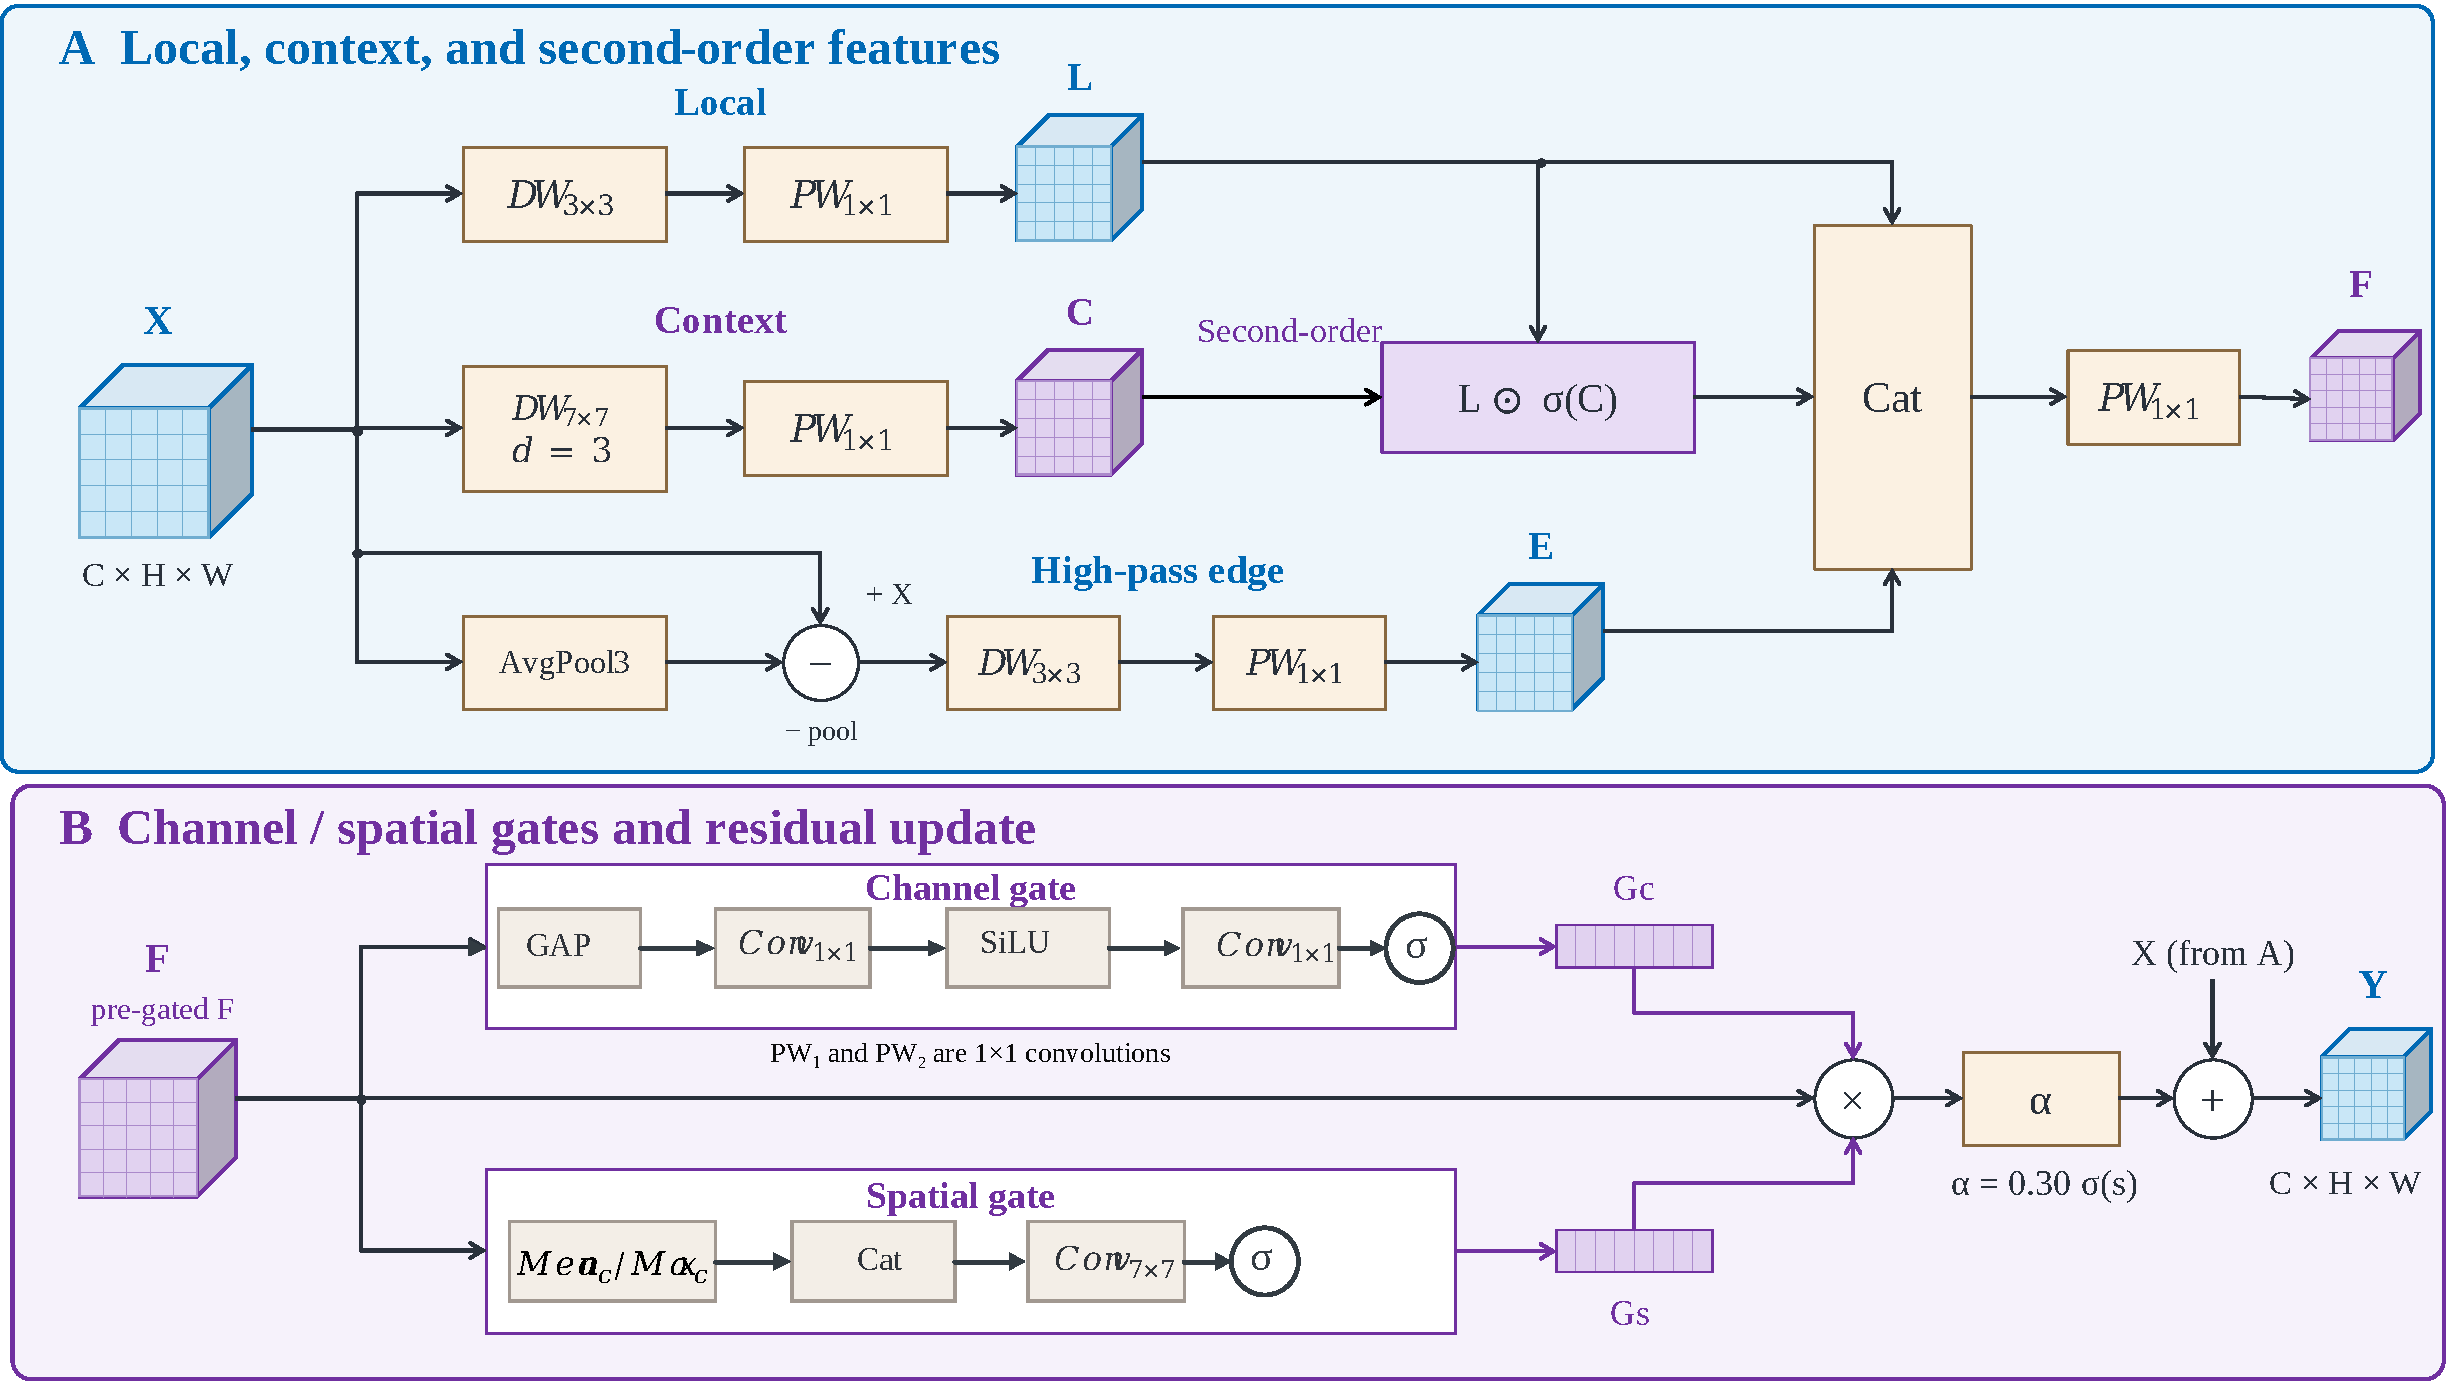
\includegraphics[width=\textwidth]{Figure_5.pdf}
\caption{High-order omni-attention (HOOA). (A) Local L, dilated-context C, and high-pass edge E branches are constructed from X. The signed subtraction ports specify X $-$ AvgPool3(X). The second-order response is L $\odot$ sigmoid(C); Cat(L, L $\odot$ sigmoid(C), E) is pointwise-projected to F. (B) Channel and spatial gates are both computed from the same pre-gated F. Their product modulates F in the residual update Y = X + $\alpha$F $\odot$ Gc $\odot$ Gs, where $\alpha$ = 0.30 sigmoid(s) is a bounded scaling coefficient. DW/PW denote depthwise/pointwise convolutions; d = 3 is the context dilation. Batch normalization and SiLU are included as specified in Methods. Tensor grids and gate vectors are schematic.}
\label{fig:figure5}
\end{figure*}



\subsection{Training objective and optimization}
\label{sec:objective}

Training combines native detection losses with configuration-specific factor/prototype supervision and an arch-position term; Mobile additionally uses a normalized Wasserstein-distance box term. With inactive terms set to zero, the objective is
\begin{equation}
 \begin{aligned}
 \mathcal L={}&\mathcal L_{\mathrm{det}}
  +\lambda_{\mathrm{arch}}\mathcal L_{\mathrm{arch}}
  +\sum_{h\in\{q,p,d\}}\lambda_h\mathcal L_{\mathrm{factor},h}\\
 &+\mathcal L_{\mathrm{proto}}
  +\lambda_{\mathrm{NWD}}\mathcal L_{\mathrm{NWD}}.
 \end{aligned}
 \label{eq:total-loss}
\end{equation}
Here the native detection objective is
\[
 \begin{aligned}
 \mathcal L_{\mathrm{det}}={}&\mathcal L_{\mathrm{MAL}}
  +5\mathcal L_{\mathrm{L1}}+2\mathcal L_{\mathrm{GIoU}}\\
 &+0.15\mathcal L_{\mathrm{FGL}}+1.5\mathcal L_{\mathrm{DDF}}.
 \end{aligned}
\]
The prototype loss in Eq.~\eqref{eq:prototype-loss} already includes its coefficient and is not weighted a second time. Intermediate-decoder and denoising supervision follow the corresponding detector implementation.

The training-only arch-position term groups matched teeth by reference vertical center, maps supported FDI identities to arch order, and penalizes the absolute difference from min--max-normalized predicted horizontal position. A small stabilizer prevents division by zero. This is a horizontal-order heuristic, not a fitted arch curve or an inference uniqueness constraint; its weights are $0.25$ for Pano/DSLR and $0.10$ for Mobile.

For Mobile, the box-distance term uses normalized center $\mathbf c$ and a normalized width--height vector $\mathbf b$ (distinct from the log-shape feature $\mathbf s$ in Eq.~\eqref{eq:geometry-features}). For each matched prediction and target,
\[
 d=\sqrt{\lVert\mathbf c-\mathbf c^*\rVert_2^2
       +\tfrac14\lVert\mathbf b-\mathbf b^*\rVert_2^2}.
\]
The implementation clamps the squared distance to at least $10^{-12}$ before taking its square root for numerical stability. Then $\mathcal L_{\mathrm{NWD}}$ is the mean of $1-\exp(-d/0.08)$, weighted by $\lambda_{\mathrm{NWD}}=0.50$. Pano and DSLR do not use this term. Factor cross-entropy weights for quadrant/position/dentition are $0.10/0.10/0.05$ in Pano and $0.08/0.08/0.03$ in Mobile.

The DSLR configuration uses the additional-decay operation of DualOpt after the ordinary AdamW step \citep{ning2026dualopt}. The extra-decay coefficient is $0.01$, the parameter-enumeration rank exponent is $1.5$, and multiplier bounds are $0.5$--$1.5$; initialization rollback is disabled.



\subsection{Query-specific attribution and judgment sensitivity}
\label{sec:visual-methods}

We complemented retrained controls with spatial attribution of selected tooth predictions. For a feature tensor $A$ and scalar query score $s$, the positive elementwise gradient--activation map is
\begin{equation}
 M_{uv}=\left[\sum_c A_{cuv}\frac{\partial s}{\partial A_{cuv}}\right]_+,
 \label{eq:cam}
\end{equation}
following the HiResCAM formulation \citep{draelos2021hirescam}. The score is the reference-FDI detection logit, or the auxiliary prototype class score where specified. Controlled CMFA and HOOA comparisons use the finest encoder output and a matched native query in each independently trained model. Final-model comparisons retain the same image, checkpoint, and query across module panels. Prototype maps explain the training branch; prototype scores remain excluded from inference fusion.

Maps were computed in FP32 on complete inputs, divided by their own positive full-image maxima, and then displayed with identical crops within each comparison. Ground-truth boxes identify and display the target tooth but do not mask the attribution. The native query-content initialization is detached, so these gradients describe the remaining differentiable paths. The maps indicate relative spatial attribution; their color intensity is not a common contribution scale across modules or models.

For the factor heads, an input-occlusion analysis \citep{zeiler2014visualizing} measures changes in the correct-factor judgment. Let $m_h(x)$ be the correct-factor logit minus the largest alternative logit in the unperturbed input for head $h$. The correct and alternative indices are held fixed. Replacing region $R$ by the image's mean RGB color gives
\begin{equation}
 \Delta_h(R)=m_h(x)-m_h(x_{\setminus R}).
 \label{eq:occlusion}
\end{equation}
Each $1024\times1024$ image is evaluated at $29\times29=841$ locations using a $128\times128$ patch and stride 32. Each perturbed forward pass yields all three heads. Encoder top-$k$ anchor indices, their order, and the target query are fixed to the baseline; feature content and downstream predictions are recomputed. The dense map averages signed margin changes over all patches covering each pixel. A symmetric raw-margin scale is shared across cases within each head. Red denotes a reduced correct-factor margin after occlusion (supporting evidence); blue denotes an increased margin (potential interference). These conditional judgment sensitivity maps are neither native attention maps nor evaluations of detection accuracy after unrestricted query reselection.

\FloatBarrier

% experiments
\section{Experiments and results}
\label{sec:experiments}

\subsection{Experimental settings}
\subsubsection{Datasets and partitions}
This retrospective computational study evaluated three acquisition-specific cohorts: the public DENTEX2023 panoramic radiography dataset \citep{hamamci2023dentex} and two private intraoral photographic datasets obtained from West China Hospital of Stomatology, Sichuan University, Chengdu, China. The private datasets comprised smartphone photographs and standardized five-view digital single-lens reflex (DSLR) photographs. DENTEX2023 uses 32 permanent-tooth FDI classes, whereas the photographic datasets use a 52-class FDI label map covering permanent and primary teeth. Dataset composition is summarized in Table~\ref{tab:table1}.

The 1,098 smartphone images were randomly divided at the image level into 878 training images and 220 validation images. Patient-level grouping was not enforced during this split. The DSLR training partition contained 750 images from 150 patients, and the validation partition contained 190 images from 38 patients. No patient was shared between the DSLR training and validation partitions. An exact decoded-pixel audit found training-image duplicates among one Pano and four Mobile validation images, and none in DSLR. A post-hoc exclusion analysis is described below; these exact-image overlaps are distinct from patient-level overlap.


% table01
\begin{table*}[pos=t,width=\textwidth]
\caption{Dataset composition of the training and validation partitions. Tooth counts refer to annotated bounding boxes.}
\label{tab:table1}
\centering
\small
\begin{tabular*}{\textwidth}{@{\extracolsep{\fill}}lrrrrr@{}}
\toprule
Cohort & Training images & Validation images & Training teeth & Validation teeth & FDI classes \\
\midrule
DENTEX2023 & 570 & 64 & 16,234 & 1,861 & 32 \\
Smartphone & 878 & 220 & 9,837 & 2,459 & 52 \\
DSLR, five-view & 750 & 190 & 10,760 & 2,742 & 52 \\
\bottomrule
\end{tabular*}
\end{table*}



\subsubsection{Implementation and design}
\label{sec:implementation}
Training used 160 epochs per run. The reported Pano and Mobile summaries use three runs selected after inspecting five completed seeds: Pano seeds 1, 3, and 4, and Mobile seeds 0, 2, and 3. They are descriptive selected-run summaries; all five runs are additionally reported in Section~\ref{sec:validation-sensitivity}. The main DSLR results summarize three reported runs. Image partitions, clinical FDI mapping, model structure, initialization source, augmentation policy, losses, and checkpoint selection were held fixed within a configuration. HGNetv2-B0 used ImageNet-pretrained backbone weights. Component ablations were trained with seed~0; within each ablation group, all settings were held fixed except for the component under investigation. The Mobile component ablations in Table~\ref{tab:table6} are reported at prototype temperature $0.50$; the separately identified archived HOOA visual comparisons use $0.20$. Intact reference models were reused where applicable, and inference-only comparisons evaluated the same checkpoint without retraining.

Training used automatic mixed precision, training and validation batch sizes of 8 and 16, gradient clipping at $0.10$, and exponential moving averages with decay $0.9999$. AdamW used learning rates of $5\times10^{-4}$ for the detector and $2.5\times10^{-4}$ for the backbone, betas $(0.9,0.999)$, and base weight decay $10^{-4}$; normalization parameters were excluded from base decay. The warm-up, flat, cosine-decay, and terminal low-learning-rate phases were retained. Geometric flips were disabled. The checkpoint with maximum validation COCO AP under each configured inference policy was selected; earlier checkpoints were retained in ties. DENT-STRIDE-Pano was selected with center and shape scoring enabled, and its subsequent prior ablation does not reselect weights. Table~\ref{tab:table2} summarizes the acquisition-specific settings.


% table02
\begin{table*}[pos=t,width=\textwidth]
\caption{Acquisition-specific configurations and component roles. Loss coefficients and augmentation probabilities refer to the evaluated models.}
\label{tab:table2}
\centering
\footnotesize
\setlength{\tabcolsep}{4pt}
\renewcommand{\arraystretch}{1.15}
\begin{tabularx}{\textwidth}{@{}p{0.265\textwidth}XXX@{}}
\toprule
Setting & Pano & Mobile & DSLR \\
\midrule
Training/evaluation input & Fixed $640\times640$ & Fixed $1024\times1024$ & Multiscale training; $640\times640$ evaluation \\
Feature processing & Base hybrid encoder & CMFA + HOOA & CMFA \\
Factor heads & Auxiliary supervision & Supervision and score fusion & Inactive \\
Prototype bank & Auxiliary supervision & Auxiliary supervision & Inactive \\
SpatialShape prior & Center + shape & Inactive & Inactive \\
Optimizer & AdamW & AdamW & AdamW + rank-dependent extra decay; no rollback \\
Mosaic / MixUp probabilities & $0\,/\,0.50$ & $0\,/\,0$ & $0\,/\,0$ \\
IoU crop / zoom-out probabilities & $0.80\,/\,0.50$ & $0.80\,/\,0.50$ & $0.80\,/\,0.50$ \\
Arch-position loss weight & $0.25$ & $0.10$ & $0.25$ \\
NWD loss weight & Inactive & $0.50$; scale $0.08$ & Inactive \\
Prototype loss weight & $0.05$ & $0.03$ & Inactive \\
Prototype temperature & $0.50$ & $0.50$ & Inactive \\
\bottomrule
\end{tabularx}
\end{table*}



Within-domain component ablations preserve their group reference's resolution, data, backbone initialization, augmentation, background losses, training budget, evaluator, and selection policy except for the stated variable. CMFA gate switches preserve output dimensions; HOOA branch switches preserve local/context processing and output projection. Factor-supervision contrasts disable factor fusion during training and inference. These controlled estimates apply to their stated reference configurations, not to every acquisition-specific configuration.

\subsubsection{Evaluation endpoints and statistics}
The primary endpoint is FDI-labelled COCO bounding-box AP over IoU thresholds $0.50{:}0.05{:}0.95$. AP50, AP75, and AR100 are secondary endpoints. Classes without validation ground truth are excluded from category averages. DEIM-family models retain the native top-300 predictions without added non-maximum suppression or an FDI-uniqueness constraint. Selected exponential-moving-average checkpoints are evaluated in FP32. Parameter counts include instantiated auxiliary heads.

At score $\geq0.30$, class-agnostic one-to-one Hungarian assignment maximizes total localization IoU; only pairs with IoU $\geq0.50$ are retained as localization matches. A correct detection additionally requires exact FDI agreement. Precision uses retained predictions, recall uses reference teeth, matched-tooth FDI accuracy uses localization matches, and localization coverage uses reference teeth as denominators. F1 is computed from pooled true positives, false positives, and false negatives within each validation cohort. Raw-query duplicate-image rate is the fraction of images containing a repeated FDI label among thresholded native outputs; it is not a clinical charting-error rate. Training variability is described by the mean and sample standard deviation (SD). For the selected Pano and Mobile runs, this SD describes the selected subset rather than variability across every completed run.


\subsubsection{Additional controlled and visual analyses}
\label{sec:additional-design}
The additional CMFA controls compare separately trained DSLR models without and with CMFA using paired seeds 0, 1, and 2 under each of two optimizer settings. One setting uses AdamW; the other uses a reference DualOpt configuration with initialization rollback weight $0.005$ and extra decay $0.01$. This second control differs from the final DSLR configuration, which disables rollback. We report within-seed AP differences and their sample SD, keeping these reference controls separate from the main framework comparison.

The Mobile prototype comparison uses seed 0 without prototype supervision versus four prototypes per class at temperature $0.50$, with prototype inference fusion disabled in both models. The HOOA visualization uses a separate seed-0 reference at temperature $0.20$, comparing full HOOA against removal of the high-pass and multiplicative second-order mechanisms while retaining its other operations. Selected examples illustrate the associated identity changes; they do not estimate the frequency of corrections. For the controlled comparison examples, predictions were retained at score $\geq0.30$ and associated with reference teeth by class-agnostic one-to-one matching at IoU $\geq0.50$. The final Mobile attribution and occlusion analyses use the same seed-2 EMA checkpoint with four prototypes per class and temperature $0.50$.

For the validation sensitivity analysis, COCO AP, AP50, AP75, and AR100 were first reproduced from saved predictions for all five completed Pano and Mobile seeds. Evaluation was then repeated after excluding validation images whose decoded RGB pixels exactly matched a training image. The retained subsets contain 63 Pano images with 1,832 tooth annotations and 216 Mobile images with 2,407 annotations, with no loss of supported FDI categories. Weights, predictions, and category mappings were unchanged; no retraining or checkpoint reselection was performed.

\subsection{Detection performance and comparisons}
\subsubsection{Detection performance and three-seed summaries}
Averaged across three seeds, the AP values were $54.205\pm0.144$, $55.459\pm0.275$, and $73.219\pm0.429$ for Pano, Mobile, and DSLR, respectively (Table~\ref{tab:table3}). Pano adopts combined center--shape scoring, Mobile uses four prototypes at temperature $0.50$, and DSLR uses CMFA with extra decay but no rollback. The corresponding AP75 values were $55.574\pm0.392$, $63.372\pm0.805$, and $83.981\pm0.318$.


% table03
\begin{table*}[pos=t,width=\textwidth]
\caption{Reported three-run summary of DENT-STRIDE validation results (mean $\pm$ sample SD). Pano and Mobile use three selected runs from five completed seeds (Section~\ref{sec:implementation}). Metrics are percentages; parameters are in millions. Each row uses the corresponding acquisition-specific DENT-STRIDE configuration.}
\label{tab:table3}
\centering
\footnotesize
\begin{tabular*}{\textwidth}{@{\extracolsep{\fill}}lrrrrr@{}}
\toprule
Configuration & AP & AP50 & AP75 & AR100 & Params (M) \\
\midrule
DENT-STRIDE-Pano & $54.205\pm0.144$ & $94.127\pm0.126$ & $55.574\pm0.392$ & $69.305\pm0.210$ & 10.650 \\
DENT-STRIDE-Mobile & $55.459\pm0.275$ & $84.008\pm0.234$ & $63.372\pm0.805$ & $69.859\pm0.661$ & 12.513 \\
DENT-STRIDE-DSLR & $73.219\pm0.429$ & $88.532\pm0.459$ & $83.981\pm0.318$ & $84.890\pm1.032$ & 11.154 \\
\bottomrule
\end{tabular*}
\end{table*}



\subsubsection{Framework-level detector comparisons}
Table~\ref{tab:table4} compares the acquisition-specific configurations with official DEIM-s, RT-DETRv2-S, and conventional detector implementations on the same cohort annotations and clinical label maps. Within each cohort, all compared methods used the same evaluation input size: $1024\times1024$ pixels for Mobile and $640\times640$ pixels for Pano and DSLR. The frameworks retained their native pretraining, training input policies, optimization, augmentation, and post-processing. External comparators include CAF-YOLO-s \citep{chen2025caf}, Dome-DETR-S \citep{hu2025dome}, and the Ultralytics YOLO implementations \citep{jocher2023ultralytics}.


% table04
\begin{table*}[pos=t,width=\textwidth]
\caption{Framework-level validation comparison. P/M/D denote Pano/Mobile/DSLR. All methods were evaluated at $1024\times1024$ pixels for Mobile and $640\times640$ pixels for Pano and DSLR; GFLOPs refer to these input sizes. Repeated-seed AP entries are mean $\pm$ sample SD; single-seed entries have no dispersion estimate. The DENT-STRIDE Pano and Mobile entries summarize the selected three runs.}
\label{tab:table4}
\centering
\footnotesize
\textbf{(a) Detection performance}\par\smallskip
\begin{tabular*}{\textwidth}{@{\extracolsep{\fill}}llrrr@{}}
\toprule
Method & Seeds & Pano AP & Mobile AP & DSLR AP \\
\midrule
Official DEIM-s & 3 & $52.827\pm0.425$ & $53.912\pm0.099$ & $72.405\pm0.202$ \\
RT-DETR-L & 1 & 51.978 & 54.718 & 73.019 \\
RT-DETRv2-S & 3 & $50.775\pm0.213$ & $50.562\pm0.486$ & $70.949\pm0.506$ \\
Faster R-CNN R50-FPN & 1 & 47.695 & 42.353 & 63.151 \\
CAF-YOLO-s & 1 & 48.058 & 46.444 & 67.460 \\
YOLOv8-s & 1 & 51.431 & 48.795 & 71.854 \\
YOLO11-s & 1 & 50.644 & 49.601 & 71.094 \\
Dome-DETR-S & 1 & 51.711 & 50.964 & 71.363 \\
DENT-STRIDE & 3 & $54.205\pm0.144$ & $55.459\pm0.275$ & $73.219\pm0.429$ \\
\bottomrule
\end{tabular*}
\par\medskip
\textbf{(b) Model size and native-forward arithmetic}\par\smallskip
\begin{tabular*}{\textwidth}{@{\extracolsep{\fill}}lrr@{}}
\toprule
Method & Params (M), P/M/D & GFLOPs, P/M/D \\
\midrule
Official DEIM-s & 10.260 / 10.286 / 10.286 & 25.145 / 60.325 / 25.237 \\
RT-DETR-L & 32.872 / 32.913 / 32.913 & 109.263 / 273.097 / 109.352 \\
RT-DETRv2-S & 20.123 / 20.149 / 20.149 & 60.994 / 153.008 / 61.083 \\
Faster R-CNN R50-FPN & 41.454 / 41.556 / 41.556 & 178.090 / 412.473 / 178.295 \\
CAF-YOLO-s & 11.501 / 11.508 / 11.508 & 27.090 / 69.398 / 27.109 \\
YOLOv8-s & 11.148 / 11.156 / 11.156 & 30.013 / 76.943 / 30.056 \\
YOLO11-s & 9.440 / 9.448 / 9.448 & 23.723 / 60.841 / 23.766 \\
Dome-DETR-S & 13.266 / 13.291 / 13.291 & 105.817 / 272.008 / 108.118 \\
DENT-STRIDE & 10.650 / 12.513 / 11.154 & 25.316 / 78.353 / 25.394 \\
\bottomrule
\end{tabular*}
\end{table*}



DENT-STRIDE-Mobile achieved a validation AP of $55.459\pm0.275$ across three seeds, compared with $53.912\pm0.099$ for official DEIM-s and $54.718$ for the single-seed RT-DETR-L reference (Fig.~\ref{fig:figure6}). The corresponding Pano AP was $54.205$, versus $52.827\pm0.425$ for official DEIM-s. DSLR achieved $73.219$ AP averaged across three seeds, exceeding the official DEIM-s mean of $72.405$ and the single-seed RT-DETR-L value of $73.019$. These descriptive rankings do not establish statistical superiority or a universal domain-independent optimum.


% figure06
\begin{figure*}[tp]
\centering
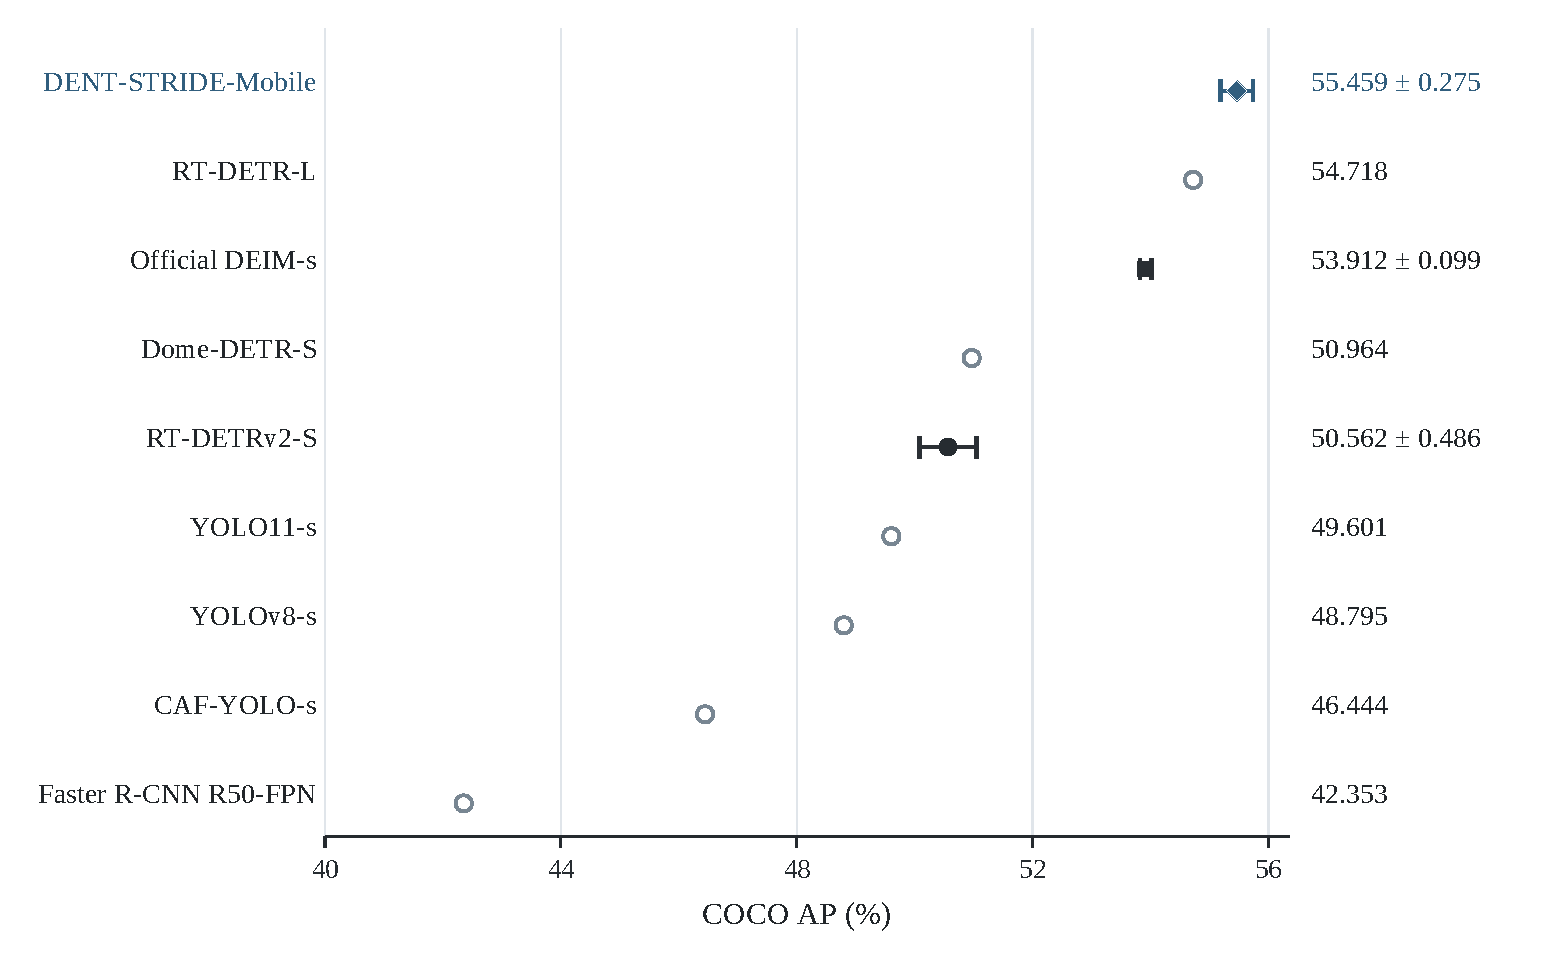
\includegraphics[width=\textwidth]{Figure_6.pdf}
\caption{Framework-level validation AP comparison on Mobile images. Filled symbols and error bars show reported three-run means and sample standard deviations; DENT-STRIDE uses the selected three Mobile runs. Open symbols denote single-run results without dispersion estimates. }
\label{fig:figure6}
\end{figure*}



\subsection{Ablation studies}
\subsubsection{Structured-identity and local-refinement branches}
Reference-configuration HOOA ablations test local-detail and context interaction in Mobile with prototype temperature $0.50$. From $55.422$ AP, removing the high-pass branch, second-order interaction, or both reduced AP to $54.511$, $53.943$, and $53.561$. With factor fusion disabled in both phases, removing quadrant, tooth-position, or dentition supervision reduced AP from $55.537$ to $54.884$, $54.263$, and $55.293$. These retrained seed-0 comparisons support the tested branches under their stated control settings. Because each ablation was evaluated with a single training seed, the results do not quantify variability in branch effects across seeds. Figure~\ref{fig:figure7} provides same-image examples from the separate archived temperature-$0.20$ HOOA reference. The complete reported component results are given in Section~\ref{sec:component-ablations}.


% figure07
\begin{figure*}[tp]
\centering
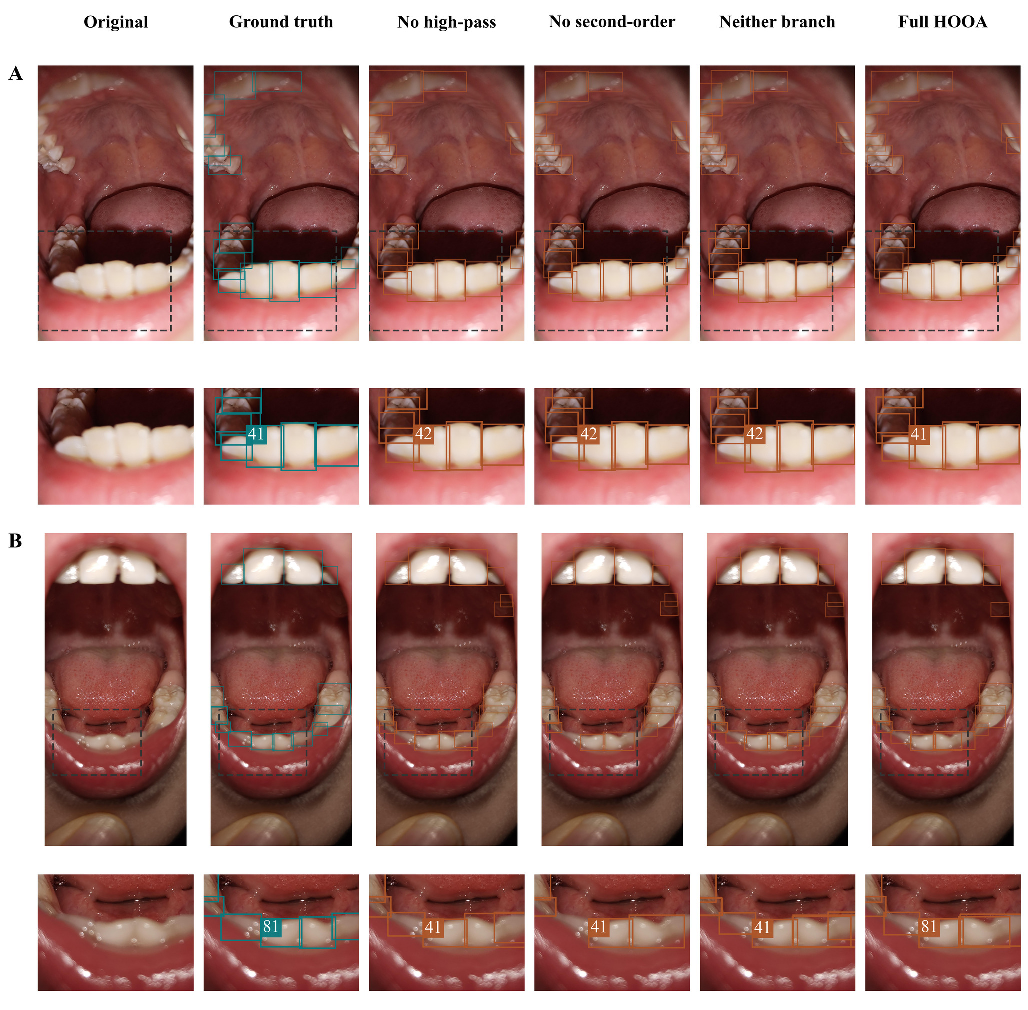
\includegraphics[width=\textwidth]{Figure_7.pdf}
\caption{HOOA branch comparison on the same smartphone images from the archived temperature-$0.20$ reference. Independently trained seed-0 models retain the same training protocol and differ only in the high-pass and second-order branches. Columns show the original image, ground truth, three branch-removal configurations, and full HOOA; lower rows show identical target enlargements. Teal boxes are ground truth and orange boxes are predictions retained at score $\geq$0.30. (A) The highlighted reference tooth is FDI 41; No high-pass: FDI 42, 14 correct matches and 7 false positives; No second-order: FDI 42, 14 correct matches and 10 false positives; Neither branch: FDI 42, 10 correct matches and 15 false positives; Full HOOA: FDI 41, 16 correct matches and 7 false positives. (B) The highlighted reference tooth is FDI 81; No high-pass: FDI 41, 10 correct matches and 9 false positives; No second-order: FDI 41, 10 correct matches and 5 false positives; Neither branch: FDI 41, 11 correct matches and 10 false positives; Full HOOA: FDI 81, 13 correct matches and 6 false positives. These selected examples illustrate branch effects in the archived reference configuration, whose full-versus-reduced AP contrast is reported in Section~\ref{sec:module-attribution}.}
\label{fig:figure7}
\end{figure*}



\subsubsection{Same-checkpoint anatomical scoring}
\label{sec:prior-ablation}
Each Pano checkpoint selected under combined center--shape scoring was evaluated with no prior, center only, shape only, or both, without reselection of weights (Table~\ref{tab:table5}; Fig.~\ref{fig:figure8}). All 300 ordinary-query boxes and their full class logits were retained before top-$k$ selection. Factor fusion, appearance scoring, and global assignment were disabled. The panoramic view term is class-constant and has no numerical effect. The comparison changes class-score ranking, not predicted box coordinates.


% table05
\begin{table*}[pos=t,width=\textwidth]
\caption{Same-checkpoint Pano anatomical scoring across the three selected seeds (1, 3, and 4). Metrics and paired AP differences versus no prior are mean $\pm$ sample SD. Metrics are percentages; AP differences are percentage points.}
\label{tab:table5}
\centering
\footnotesize
\begin{tabular*}{\textwidth}{@{\extracolsep{\fill}}lrrrrr@{}}
\toprule
Prior & AP & AP50 & AP75 & AR100 & Paired $\Delta$AP \\
\midrule
None & $53.642\pm0.119$ & $93.730\pm0.172$ & $54.592\pm0.385$ & $66.495\pm0.367$ & --- \\
Center only & $54.236\pm0.148$ & $94.195\pm0.139$ & $55.573\pm0.426$ & $69.129\pm0.232$ & $+0.595\pm0.056$ \\
Shape only & $53.679\pm0.112$ & $93.697\pm0.183$ & $54.746\pm0.354$ & $66.892\pm0.372$ & $+0.037\pm0.011$ \\
Center + shape & $54.205\pm0.144$ & $94.127\pm0.126$ & $55.574\pm0.392$ & $69.305\pm0.210$ & $+0.563\pm0.048$ \\
\bottomrule
\end{tabular*}
\end{table*}



Across three seeds, center scoring increased AP from $53.642$ to $54.236$ ($+0.595\pm0.056$ points); combined scoring reached $54.205$ ($+0.563\pm0.048$). Shape-only scoring changed AP by $+0.037\pm0.011$. AR100 averaged across three seeds was $69.129$ for center scoring and $69.305$ for combined scoring, compared with $66.495$ without a prior. Center-only scoring had the highest mean AP; combined scoring had the highest AR100, while their mean AP75 values were nearly identical. Figure~\ref{fig:figure9} shows favourable and adverse identity changes. These conditional comparisons concern inference-score effects rather than learned appearance gains.


% figure08
\begin{figure*}[tp]
\centering
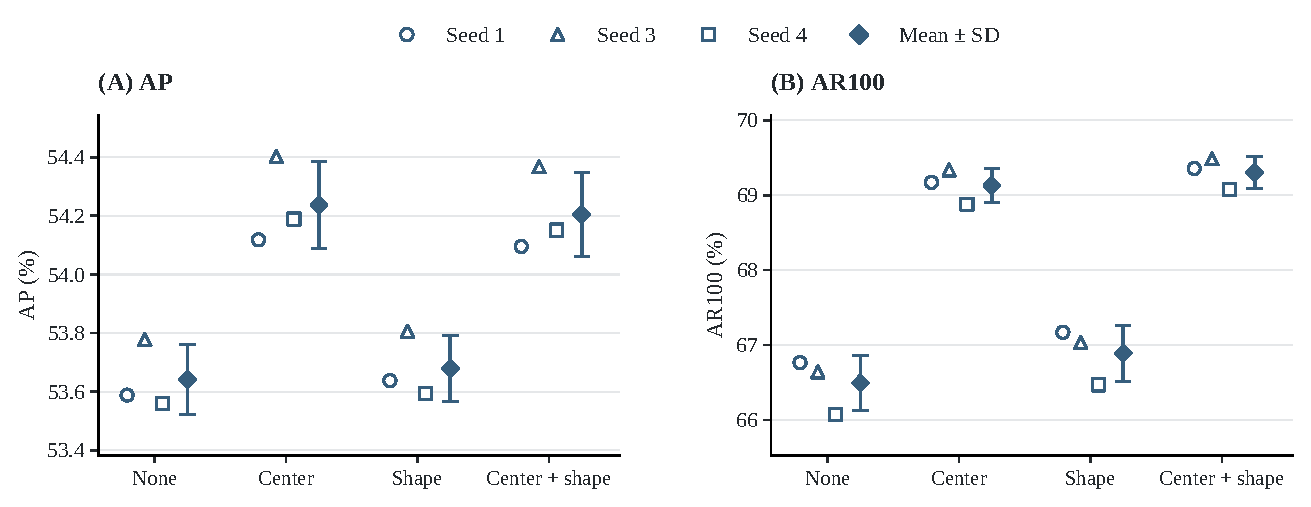
\includegraphics[width=\textwidth]{Figure_8.pdf}
\caption{Anatomical-prior scoring on DENTEX2023. Each checkpoint is evaluated with no prior, center-only, shape-only, and combined center--shape scoring from candidates before top-k selection. Open symbols denote individual seeds; filled diamonds and error bars show the mean and sample standard deviation across these three selected seeds (1, 3, and 4). (A) COCO AP. (B) AR100. Relative to no prior, center-only, shape-only, and combined scoring change mean AP by +0.595, +0.037, and +0.563 percentage points, respectively. Weights are fixed within each seed; therefore, the comparison isolates inference scoring rather than training effects. }
\label{fig:figure8}
\end{figure*}



% figure09
\begin{figure*}[tp]
\centering
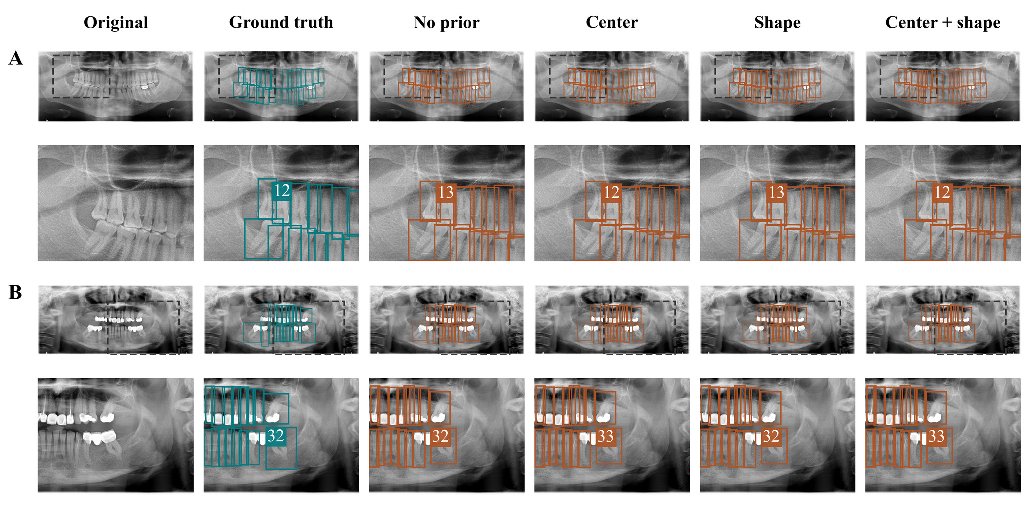
\includegraphics[width=\textwidth]{Figure_9.pdf}
\caption{Same-weight DENTEX anatomical-prior comparison using the representative seed-3 checkpoint. The four scoring conditions use no prior, center only, shape only, and center plus shape. Scores are recomputed before native top-300 selection and box coordinates are unchanged. Teal boxes denote ground truth and orange boxes predictions retained at score $\geq$0.30; lower rows show identical target enlargements. (A) At the same query box, the highest retained label changes from FDI 13 to FDI 12 for reference FDI 12; image-level correct matches change from 25 to 26. (B) At the same query box, the highest retained label changes from FDI 32 to FDI 33 for reference FDI 32; image-level correct matches change from 18 to 17. The favorable and adverse examples illustrate score-ranking effects, not changes in learned localization.}
\label{fig:figure9}
\end{figure*}



\subsubsection{Component ablations}
\label{sec:component-ablations}
Table~\ref{tab:table6} reports the reference-configuration feature-gating, HOOA-branch, and factor-supervision ablations. Figure~\ref{fig:figure10} summarizes the HOOA and factor-supervision contrasts. Among the tested CMFA gate settings, the both-gates configuration achieved the highest AP ($55.422$), followed by channel-only ($54.810$), spatial-only ($54.428$), and neither gate ($54.383$). These comparisons were obtained from single-seed experiments.


% table06
\begin{table*}[pos=t,width=\textwidth]
\caption{Reference-configuration seed-0 feature-gating, HOOA-branch, and factor-supervision ablations. $\Delta$AP subtracts the stated group reference; factor-supervision models disable training and inference fusion. Learning controls are separately trained except for reused intact references. Metrics are percentages; AP differences are percentage points.}
\label{tab:table6}
\centering
\footnotesize
\setlength{\tabcolsep}{4pt}
\renewcommand{\arraystretch}{1.12}
\begin{tabularx}{\textwidth}{@{}lXrrrrr@{}}
\toprule
Component & Setting & AP & AP50 & AP75 & AR100 & $\Delta$AP \\
\midrule
CMFA gates & Both gates & 55.422 & 84.340 & 62.160 & 68.519 & $+0.000$ \\
 & Channel only & 54.810 & 83.574 & 60.104 & 69.350 & $-0.612$ \\
 & Spatial only & 54.428 & 83.603 & 60.809 & 69.803 & $-0.994$ \\
 & Neither & 54.383 & 83.425 & 60.625 & 68.219 & $-1.039$ \\
\midrule
HOOA branches & Full HOOA & 55.422 & 84.340 & 62.160 & 68.519 & $+0.000$ \\
 & Without high-pass & 54.511 & 83.607 & 61.141 & 69.371 & $-0.911$ \\
 & Without second-order & 53.943 & 82.951 & 59.354 & 68.935 & $-1.479$ \\
 & Without both & 53.561 & 83.010 & 58.835 & 68.556 & $-1.861$ \\
\midrule
Factor supervision & All three factors; train/inference fusion off & 55.537 & 84.951 & 62.152 & 68.431 & $+0.000$ \\
 & Without quadrant & 54.884 & 83.689 & 59.929 & 66.771 & $-0.654$ \\
 & Without position & 54.263 & 82.904 & 59.844 & 66.052 & $-1.274$ \\
 & Without dentition & 55.293 & 83.806 & 63.188 & 68.188 & $-0.244$ \\
\bottomrule
\end{tabularx}
\end{table*}



% figure10
\begin{figure*}[tp]
\centering
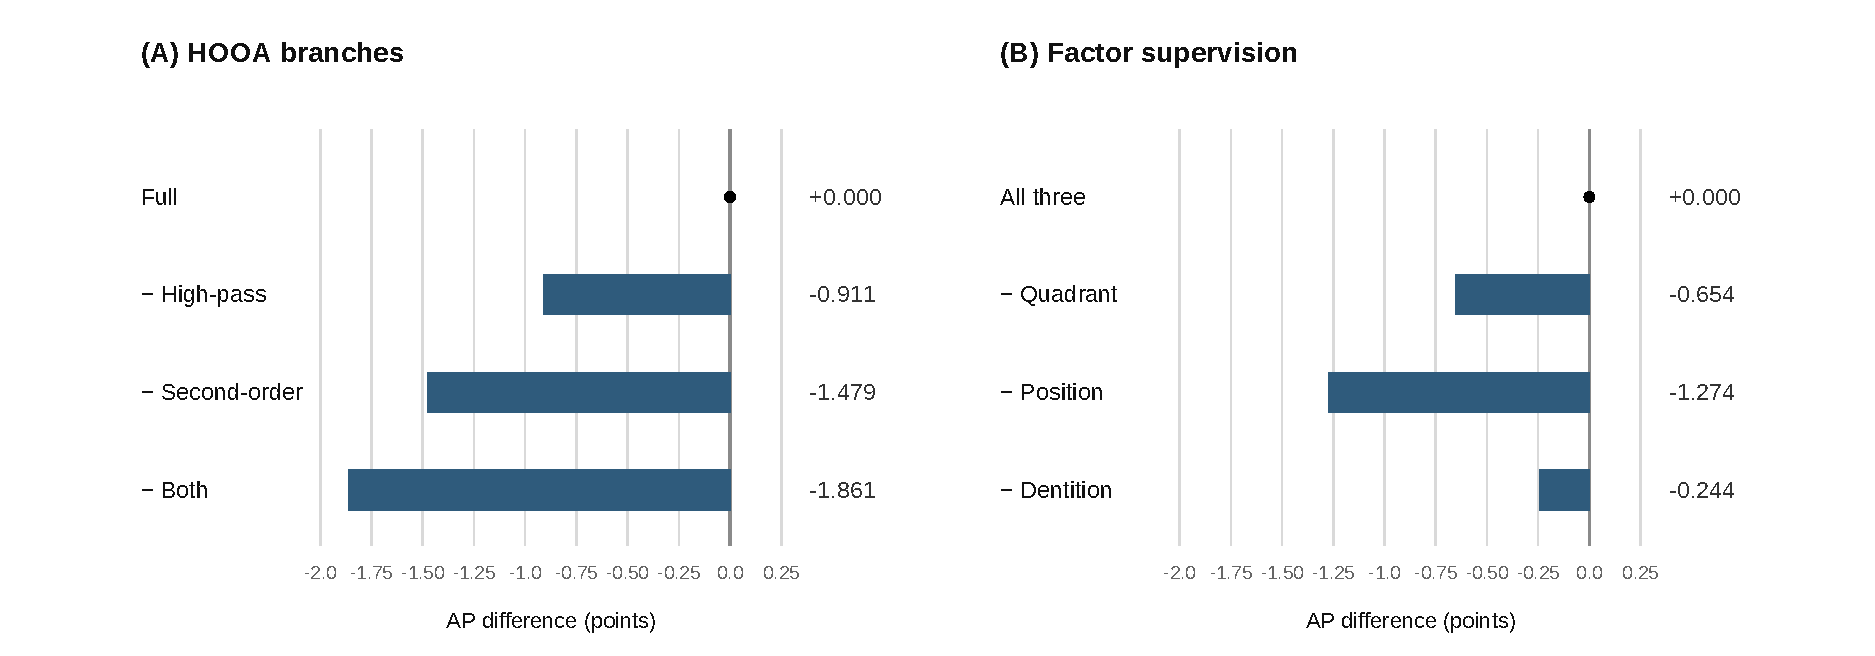
\includegraphics[width=\textwidth]{Figure_10.pdf}
\caption{Retrained HOOA and factor-supervision ablations. Bars report AP differences after each branch or supervision-target removal. HOOA comparisons use the HOOA-group seed-0 reference with all HOOA branches enabled (55.422 AP); factor supervision uses all three targets with training and inference fusion disabled (55.537 AP). Every tested removal is shown. These single-seed results have no uncertainty bars.}
\label{fig:figure10}
\end{figure*}



\subsection{Further analyses}
\subsubsection{Tooth identity and numbering consistency}
Table~\ref{tab:table7} reports the fixed-threshold endpoints for the three-seed groups. Mean F1 was $89.346\%$, $80.732\%$, and $92.841\%$ for Pano, Mobile, and DSLR, respectively. Matched-tooth FDI accuracy was $92.843\%$, $92.054\%$, and $97.451\%$, whereas raw-query duplicate-image rates were $45.312\%$, $36.970\%$, and $22.982\%$. High conditional identity accuracy therefore coexists with repeated labels at image level.


% table07
\begin{table*}[pos=t,width=\textwidth]
\caption{Fixed-threshold endpoints for the three-seed summary groups in Table~\ref{tab:table3} (mean $\pm$ sample SD), at score $\geq0.30$ and localization IoU $\geq0.50$. Values are percentages. FDI accuracy uses localization matches; recall and coverage use reference teeth; duplicate-image rate uses all images.}
\label{tab:table7}
\centering
\footnotesize
\setlength{\tabcolsep}{3pt}
\begin{tabular*}{\textwidth}{@{\extracolsep{\fill}}lrrrrrr@{}}
\toprule
Cohort & Precision & Recall & F1 & \shortstack{Matched-tooth\\FDI accuracy} & \shortstack{Localization\\coverage} & \shortstack{Duplicate\\images} \\
\midrule
Pano & $87.250\pm0.658$ & $91.546\pm0.324$ & $89.346\pm0.467$ & $92.843\pm0.311$ & $98.603\pm0.054$ & $45.312\pm5.634$ \\
Mobile & $74.951\pm1.736$ & $87.488\pm0.778$ & $80.732\pm1.304$ & $92.054\pm0.547$ & $95.039\pm0.285$ & $36.970\pm4.074$ \\
DSLR & $90.941\pm0.431$ & $94.821\pm0.435$ & $92.841\pm0.433$ & $97.451\pm0.310$ & $97.301\pm0.138$ & $22.982\pm1.325$ \\
\bottomrule
\end{tabular*}
\end{table*}



Figure~\ref{fig:figure11} compares the same images across official DEIM-s, RT-DETR-L, and DENT-STRIDE with consistent thresholds and shared local enlargements. For qualitative comparisons, representative archived checkpoints were selected by validation AP within their respective run groups (Mobile seed 2; Pano and DSLR seed 3).


% figure11
\begin{figure*}[p]
\centering
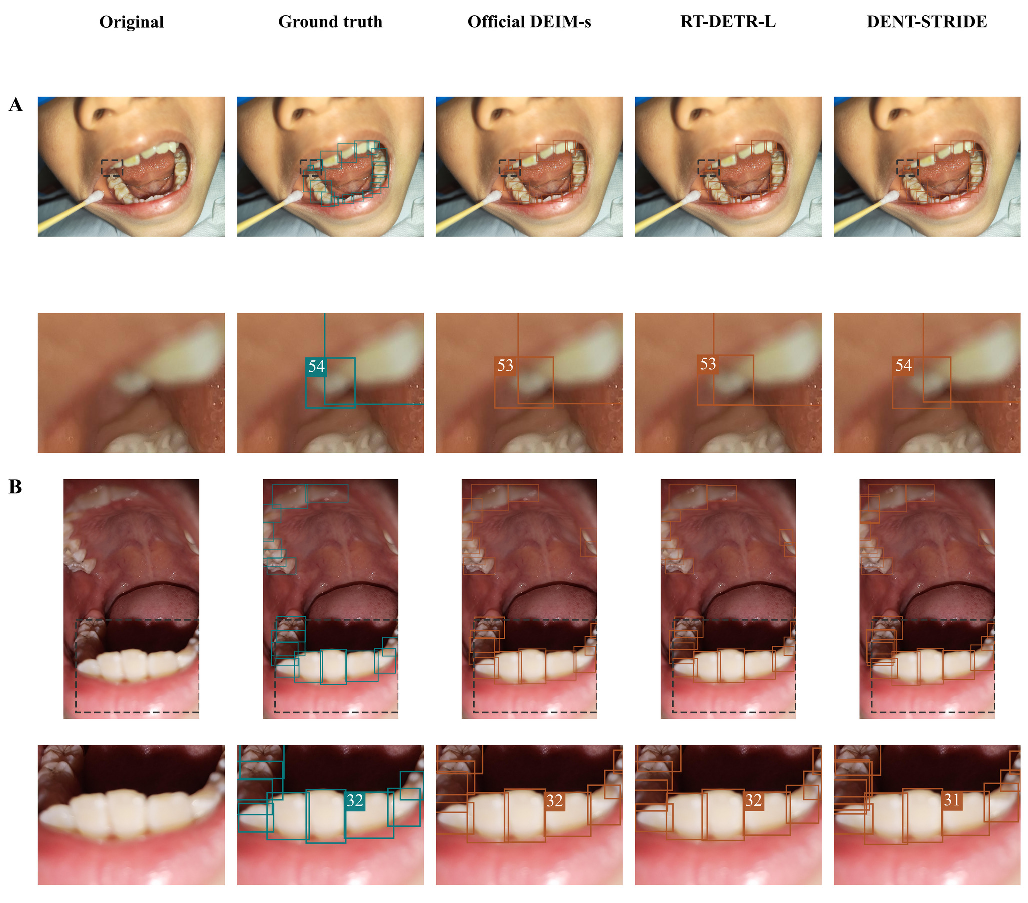
\includegraphics[width=\textwidth]{Figure_11A.pdf}
\caption{\textbf{A. Mobile cohort.} Same-image Mobile detector comparison using the representative DENT-STRIDE seed-2 checkpoint. Columns show original image, ground truth, official DEIM-s, RT-DETR-L, and DENT-STRIDE; lower rows share identical target enlargements. Teal denotes ground truth and orange predictions retained at score $\geq$0.30. (A) Reference FDI 54; Official DEIM-s: FDI 53, 16 correct matches and 5 false positives; RT-DETR-L: FDI 53, 16 correct matches and 7 false positives; DENT-STRIDE: FDI 54, 18 correct matches and 4 false positives. (B) Reference FDI 32; Official DEIM-s: FDI 32, 16 correct matches and 5 false positives; RT-DETR-L: FDI 32, 14 correct matches and 11 false positives; DENT-STRIDE: FDI 31, 11 correct matches and 15 false positives. Frameworks retain their native training and output-processing settings. Improvement and adverse examples are illustrative and do not estimate population frequencies.}
\label{fig:figure11}
\label{fig:figure11a}
\end{figure*}

\begin{figure*}[p]
\ContinuedFloat
\centering
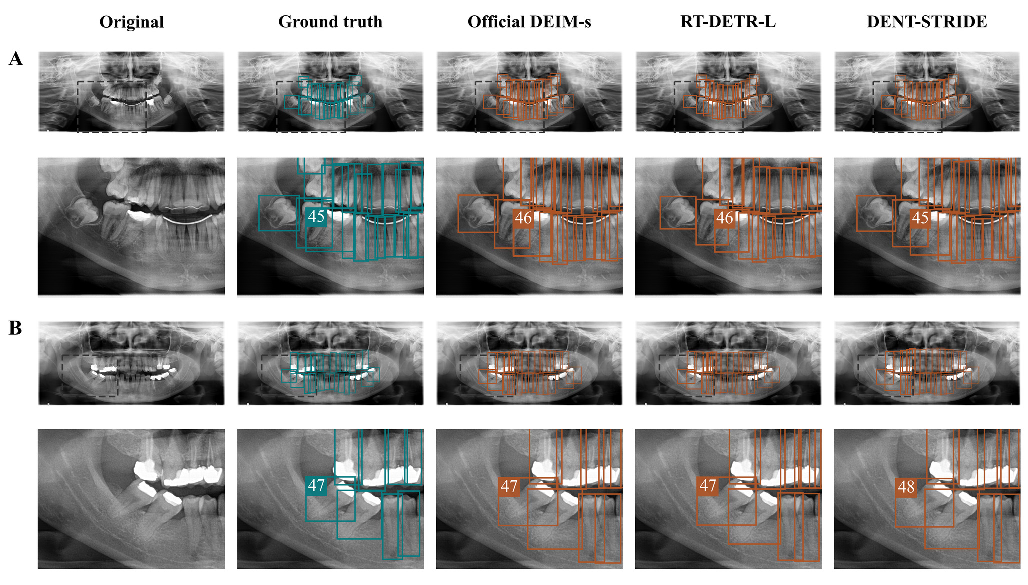
\includegraphics[width=\textwidth]{Figure_11B.pdf}
\caption{\textbf{B. Panoramic cohort.} Same-image panoramic detector comparison using the representative DENT-STRIDE seed-3 checkpoint. Columns show original image, ground truth, official DEIM-s, RT-DETR-L, and DENT-STRIDE; lower rows share identical target enlargements. Teal denotes ground truth and orange predictions retained at score $\geq$0.30. (A) Reference FDI 45; Official DEIM-s: FDI 46, 18 correct matches and 23 false positives; RT-DETR-L: FDI 46, 18 correct matches and 19 false positives; DENT-STRIDE: FDI 45, 20 correct matches and 15 false positives. (B) Reference FDI 47; Official DEIM-s: FDI 47, 28 correct matches and 2 false positives; RT-DETR-L: FDI 47, 28 correct matches and 4 false positives; DENT-STRIDE: FDI 48, 25 correct matches and 6 false positives. Frameworks retain their native training and output-processing settings. Improvement and adverse examples are illustrative and do not estimate population frequencies.}
\label{fig:figure11b}
\end{figure*}

\begin{figure*}[p]
\ContinuedFloat
\centering
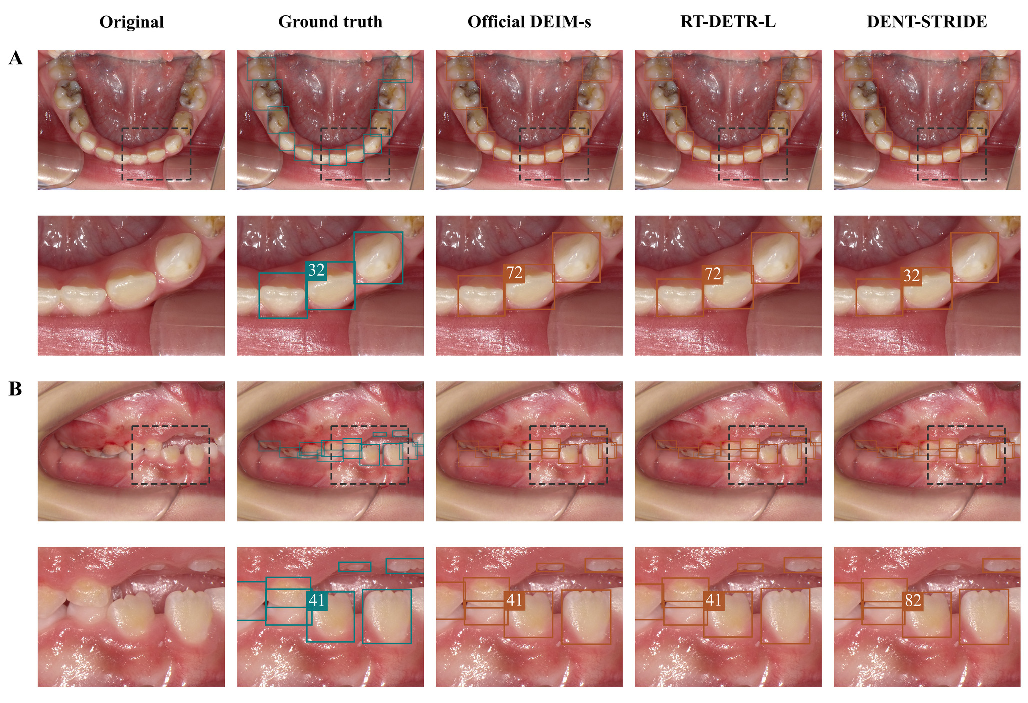
\includegraphics[width=\textwidth]{Figure_11C.pdf}
\caption{\textbf{C. DSLR cohort.} Same-image DSLR detector comparison using the representative DENT-STRIDE seed-3 checkpoint. Columns show original image, ground truth, official DEIM-s, RT-DETR-L, and DENT-STRIDE; lower rows share identical target enlargements. Teal denotes ground truth and orange predictions retained at score $\geq$0.30. (A) Reference FDI 32; Official DEIM-s: FDI 72, 8 correct matches and 7 false positives; RT-DETR-L: FDI 72, 7 correct matches and 10 false positives; DENT-STRIDE: FDI 32, 9 correct matches and 6 false positives. (B) Reference FDI 41; Official DEIM-s: FDI 41, 14 correct matches and 8 false positives; RT-DETR-L: FDI 41, 13 correct matches and 10 false positives; DENT-STRIDE: FDI 82, 10 correct matches and 13 false positives. Frameworks retain their native training and output-processing settings. Improvement and adverse examples are illustrative and do not estimate population frequencies.}
\label{fig:figure11c}
\end{figure*}




\subsubsection{Paired CMFA controls and prototype supervision}
\label{sec:controlled-additional}
Figure~\ref{fig:figure12} summarizes the additional controlled comparisons. Enabling CMFA increased DSLR AP in every paired seed: the changes were $+0.492$, $+0.357$, and $+0.647$ points with AdamW, averaging $+0.498\pm0.145$. Under the reference DualOpt setting with rollback, the corresponding gains were $+0.545$, $+0.411$, and $+0.584$ points, averaging $+0.513\pm0.091$. The consistent AP direction across these pairs supports cross-scale aggregation in the tested settings; secondary endpoints did not improve uniformly in every pair. The Mobile seed-0 prototype control increased AP from $54.918$ to $55.683$ ($+0.765$ points), supporting auxiliary identity supervision without adding prototype scores at inference.

\begin{figure*}[tp]
\centering
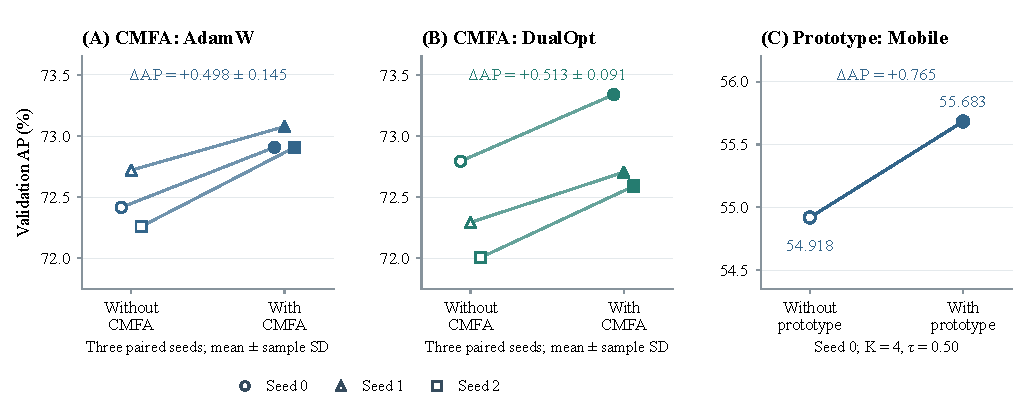
\includegraphics[width=\textwidth]{Figure_12.pdf}
\caption{Controlled effects of CMFA and prototype supervision. (A,B) Matched DSLR AP values without and with CMFA for seeds 0, 1, and 2 under AdamW and reference DualOpt with rollback. Lines connect the same seed; the annotations report mean paired AP gain and sample SD. The reference DualOpt setting includes rollback and differs from the final DSLR optimizer. (C) Mobile AP without and with prototype supervision at seed 0; no between-seed error bar is available for this contrast. All differences are AP percentage points.}
\label{fig:figure12}
\end{figure*}

\subsubsection{Identity corrections and module attribution}
\label{sec:module-attribution}
In the prototype example (Fig.~\ref{fig:figure13}), the reference primary tooth FDI 51 is predicted as permanent tooth FDI 11 without prototype supervision and correctly as 51 after it is enabled. The auxiliary prototype CAM and supported-class scores connect this correction with the supervised identity representation. The displayed LogSumExp scores are unnormalized class scores, not probabilities. Inspection of the final Mobile seed-2 bank found nearly collinear same-class vectors across the 48 supported classes (mean within-class pairwise cosine similarity $0.999999965$). Thus, the positive controlled result supports prototype-assisted identity supervision, without implying that the four slots encode four distinct tooth morphologies.

\begin{figure*}[tp]
\centering
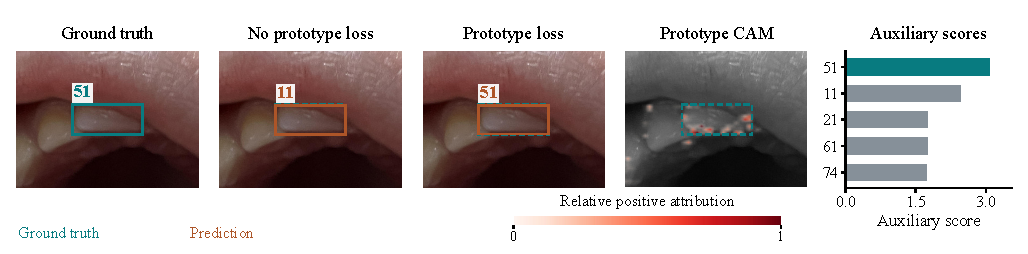
\includegraphics[width=\textwidth]{Figure_13.pdf}
\caption{Prototype-assisted identity supervision for reference FDI 51 (Mobile image 44). Independently trained seed-0 models change the matched prediction from FDI 11 to 51 when prototype supervision is enabled. The bank uses four prototypes per class at temperature $0.50$, with inference fusion disabled. The prototype CAM targets the auxiliary class score; the final panel gives the five highest supported-class LogSumExp scores. Teal boxes denote ground truth and orange boxes predictions. CAMs follow Eq.~\eqref{eq:cam}, with independent full-image normalization before the same crop; dashed reference boxes do not mask the maps.}
\label{fig:figure13}
\end{figure*}

The separate HOOA reference comparison at temperature $0.20$ increased AP from $53.561$ to $54.910$ when the high-pass and second-order mechanisms were retained ($+1.349$ points). Figure~\ref{fig:figure14} shows the accompanying FDI 53-to-13 correction for a reference permanent canine. In this example, the positive reference-class attribution is more concentrated near the target tooth with full HOOA. This contrast tests two mechanisms within HOOA, rather than removing the entire module.

\begin{figure*}[tp]
\centering
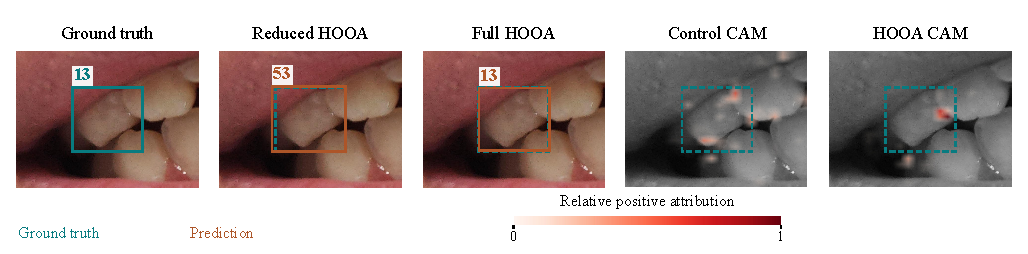
\includegraphics[width=\textwidth]{Figure_14.pdf}
\caption{HOOA mechanism comparison for reference FDI 13 (Mobile image 77). The reduced model removes the high-pass response and substitutes the direct context response for the multiplicative second-order response; other HOOA operations remain active. Full HOOA corrects FDI 53 to 13. Both models use seed 0 and prototype temperature $0.20$. CAMs target the reference-FDI detection logit at the finest encoder output, using an independently matched query in each model. Boxes and per-map normalization follow Fig.~\ref{fig:figure13}.}
\label{fig:figure14}
\end{figure*}

The DSLR CMFA examples in Fig.~\ref{fig:figure15} show corrections from FDI 55 to 16 and from 81 to 41 under the AdamW seed-0 control. These cases illustrate the identity changes underlying the paired comparison without requiring every corrected prediction to have a more spatially concentrated CAM. Their attribution patterns include both the target tooth and adjacent image context.

\begin{figure*}[tp]
\centering
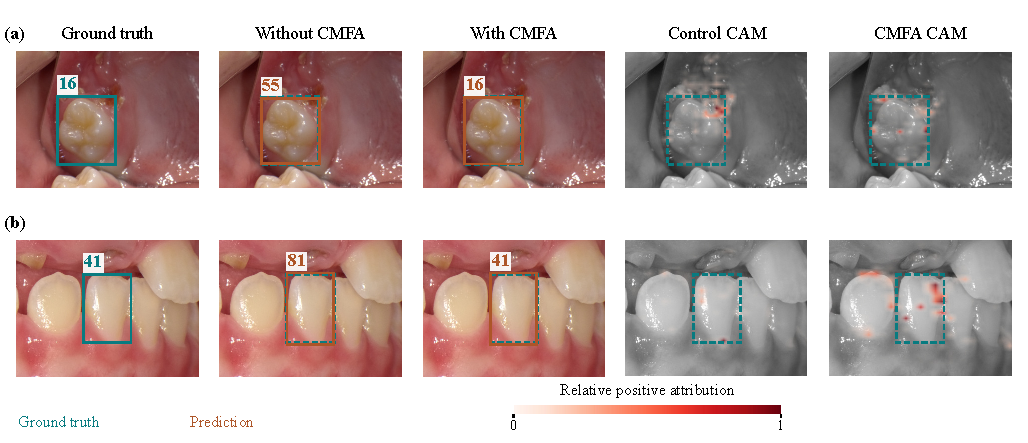
\includegraphics[width=\textwidth]{Figure_15.pdf}
\caption{CMFA controls on two DSLR images with AdamW and seed 0. Reference teeth are (a) FDI 16 in image 125 and (b) FDI 41 in image 124. Enabling CMFA corrects the matched labels from FDI 55 to 16 and from 81 to 41. CAMs target the reference-FDI detection logit at the finest encoder output using independently matched native queries. Boxes and normalization follow Fig.~\ref{fig:figure13}; intensity cannot be compared as a contribution magnitude between models. The paired validation gains are shown in Fig.~\ref{fig:figure12}.}
\label{fig:figure15}
\end{figure*}

Figure~\ref{fig:figure16} then examines the final Mobile model on a partly visible tooth and a blurred image. Within each row, detection, CMFA, and HOOA high-pass maps explain the same reference-FDI detection logit, while the prototype map explains the auxiliary identity score. All panels use the same checkpoint, image, and native query. The different spatial patterns provide complementary views of the executed feature and identity pathways; they are mechanism illustrations rather than additional ablations.

\begin{figure*}[tp]
\centering
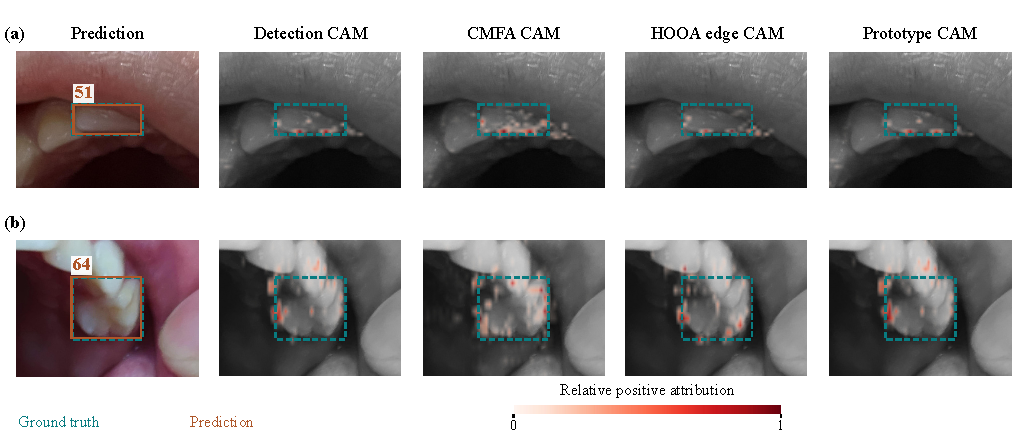
\includegraphics[width=\textwidth]{Figure_16.pdf}
\caption{Module attribution in the final Mobile model (EMA seed 2; four prototypes; temperature $0.50$). Rows show (a) partly visible FDI 51 in image 44 and (b) FDI 64 in blurred image 115. Each row uses one image, checkpoint, and native query. Detection, CMFA, and HOOA edge maps target the reference-FDI detection logit at the finest encoder output, finer top-down fusion output, and high-pass branch tensor, respectively. The prototype map targets the auxiliary class score, excluded from inference fusion. Each map is normalized by its own full-image maximum before cropping. Orange boxes are predictions and dashed teal boxes are reference locations.}
\label{fig:figure16}
\end{figure*}

\subsubsection{Factor-head judgment sensitivity}
Figure~\ref{fig:figure17} shows the input-occlusion results for reference teeth FDI 64, 11, and 46. Quadrant and dentition judgments show supportive regions near the target teeth; position judgments also respond to surrounding teeth and context. Across these selected cases, the patch producing the largest correct-margin decrease intersects the target box for every head. Signed changes reveal both supportive regions and regions whose occlusion increases the correct margin. The maps therefore identify where the fixed-query judgments depend on input evidence, complementing the factor-supervision controls. Ground-truth boxes were used for correspondence and display, not to generate hotspots.

\begin{figure*}[tp]
\centering
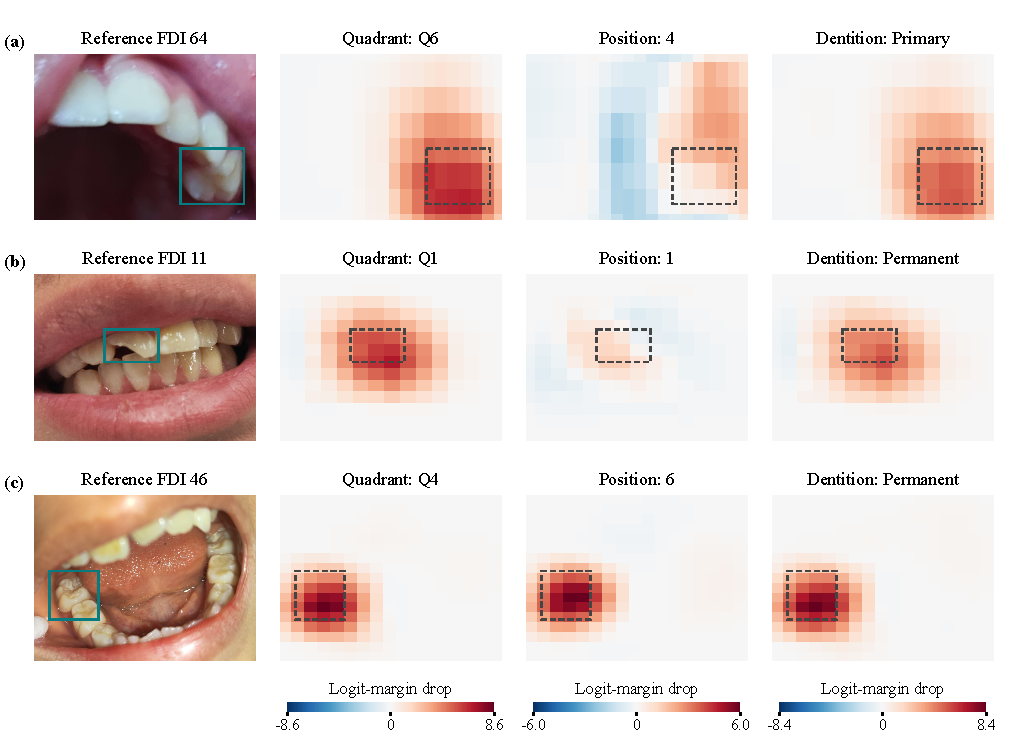
\includegraphics[width=\textwidth]{Figure_17.pdf}
\caption{Judgment sensitivity maps for the quadrant, position, and dentition heads in the final Mobile model. Rows correspond to reference FDI 64, 11, and 46. Each image undergoes 841 mean-RGB occlusions ($128\times128$ pixels; stride 32 on a $1024\times1024$ input), with all three heads evaluated in each pass. Red indicates that occlusion weakens the correct-factor logit margin; blue indicates that it strengthens the margin. Dense maps average signed changes over overlapping patches. Each head shares one symmetric raw-margin scale across cases. Baseline anchor indices, their order, and the target query are fixed while input-dependent content and downstream predictions are recomputed. Dashed boxes mark reference teeth and do not mask the calculation. These are conditional sensitivity maps, not native attention or probability maps.}
\label{fig:figure17}
\end{figure*}


\subsubsection{All-run and exact-duplicate sensitivity}
\label{sec:validation-sensitivity}
Across all five completed runs, original-split AP was $53.979\pm0.337$ for Pano and $55.292\pm0.301$ for Mobile, compared with the selected-three means of $54.205\pm0.144$ and $55.459\pm0.275$. Figure~\ref{fig:figure18} displays every seed and identifies the runs used in the reported three-run summaries. After excluding exact training-image duplicates from validation, all-five AP was $54.558\pm0.428$ for Pano and $55.039\pm0.319$ for Mobile. The paired changes averaged $+0.579\pm0.132$ and $-0.253\pm0.031$ points, respectively. The direction of sensitivity therefore differed between cohorts. These results describe unchanged checkpoints on restricted validation subsets and do not estimate performance after retraining on independently defined partitions.

\begin{figure*}[tp]
\centering
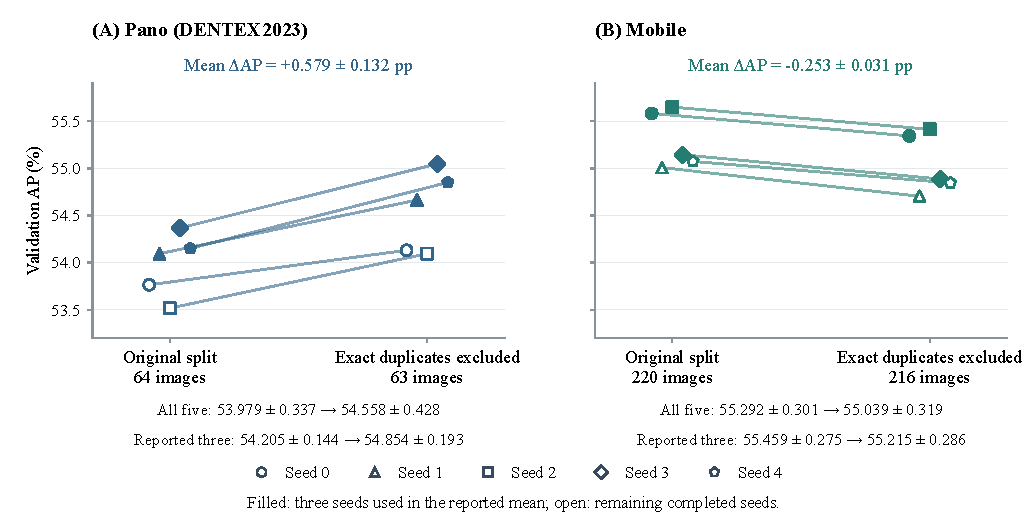
\includegraphics[width=\textwidth]{Figure_18.pdf}
\caption{Post-hoc sensitivity to exact training/validation image overlap, showing all five completed seeds. (A) Pano: 64 original validation images versus 63 after excluding one exact training-image duplicate. (B) Mobile: 220 original images versus 216 after excluding four duplicates. Lines connect unchanged checkpoints from the same seed. Filled symbols identify the three runs included in the reported mean; open symbols identify the other completed runs. Text gives AP mean $\pm$ sample SD for all five and for the reported three. The displayed $\Delta$AP is the mean $\pm$ sample SD of the five paired changes, in percentage points. Original metrics were reproduced from saved predictions before exclusion. No retraining or checkpoint reselection was performed.}
\label{fig:figure18}
\end{figure*}

\subsubsection{Computational cost}

Table~\ref{tab:table8} summarizes model size and native-forward arithmetic. The Pano, Mobile, and DSLR native forwards require approximately $12.587$, $38.938$, and $12.633$ tool-counted GMACs, respectively, at their stated evaluation resolutions. Parameters include instantiated auxiliary heads. Prototype tensor contractions are counted in the profiler's FLOP total but not its MAC total; consequently, FLOPs are not exactly twice MACs. These counts exclude post-processing and uninstrumented operations, including deformable-attention grid sampling, and are not latency or memory benchmarks.


% table08
\begin{table*}[pos=t,width=\textwidth]
\caption{Model size and tool-counted native-forward arithmetic for the domain configurations. Measurements use calflops 0.3.2, batch size 1, FP32, and evaluation mode, including auxiliary outputs. Post-processing and unsupported operations are excluded.}
\label{tab:table8}
\centering
\small
\begin{tabular*}{\textwidth}{@{\extracolsep{\fill}}llrrr@{}}
\toprule
Configuration & Evaluation input & Params (M) & GMACs & GFLOPs \\
\midrule
DENT-STRIDE-Pano & $640\times640$ & 10.650 & 12.587 & 25.316 \\
DENT-STRIDE-Mobile & $1024\times1024$ & 12.513 & 38.938 & 78.353 \\
DENT-STRIDE-DSLR & $640\times640$ & 11.154 & 12.633 & 25.394 \\
\bottomrule
\end{tabular*}
\end{table*}




% discussion
\section{Discussion}
\label{sec:discussion}

\subsection{Principal findings}

DENT-STRIDE separates identity learning, feature refinement, and anatomical score correction within an acquisition-configured detector. The reported standard deviations describe dispersion among the runs included in each summary; the all-five analyses characterize the completed Pano and Mobile runs.  Center scoring improved Pano AP at all checkpoints; shape-only effects were small and positive, while joint scoring had the highest AR100. The additional CMFA controls show positive paired AP changes in all three seeds under both reference optimizers, while the seed-0 prototype comparison supports auxiliary identity supervision. Together, these experiments support the tested feature, identity, and anatomical-scoring mechanisms within their respective configurations.

Earlier label-tree and prior-knowledge systems encode tooth identity and anatomy \citep{zhang2018labeltree,ali2023teeth}. DENT-STRIDE places factor-score fusion and training-derived geometry within a common query detector and separates their training and inference roles. Center and shape templates do not change learned query representations or predicted boxes. In the representative Mobile bank, the four within-class prototypes are almost coincident; their high cosine cohesion is therefore not evidence of four distinct morphological modes. The seed-0 controlled gain and the seed-2 bank diagnostic support auxiliary identity supervision without establishing distinct same-class morphological modes. The selected CAM examples connect aggregate effects to actual identity corrections, and the input-occlusion maps independently show spatial sensitivity of the factor judgments.

\subsection{Acquisition dependence and clinical interpretation}

Panoramic framing provides a stable reference for the training-derived center templates in Fig.~\ref{fig:figure3}. In photographic images, local appearance, occlusion, similar neighbouring teeth, and mixed dentition motivate structured identity targets and multiscale feature processing. Domain-specific input, augmentation, background losses, and inference settings form part of the evaluated system, rather than interchangeable implementation details. The Mobile framework comparison therefore cannot attribute its AP difference exclusively to identity learning.

Conditional FDI accuracy does not ensure globally unique numbering. The duplicate-image endpoint and selected failure examples expose the remaining separation between tooth-level detection and chart consistency. Clinical interpretation also requires accounting for missing teeth, overlapping views, mixed dentition, and uncertainty.

\subsection{Limitations}

The reported standard deviations describe dispersion among the included runs, not patient-level uncertainty. The Pano and Mobile three-run summaries were selected after inspecting five completed runs; the all-five results make the effect of this selection explicit. Exclusion of the identified exact training-image duplicates changed AP in opposite directions across the two cohorts, but this post-hoc analysis retains the original model-selection history and cannot rule out near duplicates or unidentified patient overlap. The smartphone split was performed at the image level without enforced patient grouping, so potential patient overlap may lead to optimistic estimates of generalization. The DSLR partitions were patient-disjoint, but the photographic cohorts originated from a single institution. Moreover, checkpoints were selected by validation AP and results were reported on those validation partitions. These results therefore do not establish performance on an independent test cohort or at an external institution.

The HOOA, factor-supervision, and prototype controls use one seed, whereas the additional CMFA comparisons use three paired seeds per reference optimizer. Prior comparisons remain conditional on weights obtained under combined scoring. Selected attribution examples do not quantify correction prevalence; the gradient maps follow the available differentiable paths, and mean-color occlusion introduces an artificial perturbation. External systems retain framework-specific pretraining, input policies, optimization, and post-processing. Unsupported prototype slots cannot be interpreted as learned class evidence, and nearly coincident same-class prototypes do not establish multimodal representation. No clinician reader or confidence-calibration study was performed. Patient-disjoint external evaluation, calibration analysis, and explicit assessment of complete-chart consistency are needed to establish the clinical scope of the approach.



\FloatBarrier

% conclusion
\section{Conclusion}
\label{sec:conclusion}

DENT-STRIDE combines explicit FDI identity supervision, acquisition-specific feature processing, and separate training-derived anatomical scoring. Across the three reported runs, mean validation AP was $54.205\pm0.144$, $55.459\pm0.275$, and $73.219\pm0.429$ for panoramic, smartphone, and DSLR images, respectively. Reference-configuration HOOA and factor-supervision controls, paired CMFA gains, prototype supervision, and same-weight center-prior comparisons provide mechanism-specific evidence. Query-specific attribution and factor-head judgment sensitivity connect these controlled results to the spatial evidence used in selected tooth decisions. The observed tooth-level accuracy and remaining repeated labels support further evaluation of numbering consistency and patient-independent generalization before clinical deployment.



% declarations
\section*{Acknowledgements}

The authors thank Haiyue Lan, Jinlin Guo, Hequan Wen, Dongxia Hu, Yuzhuo Zhang, and Yutian Li for their contributions to image annotation.

\section*{Funding and declaration of competing interest}

This work was supported in part by the Health Planning Committee of Sichuan (19PJ074 to R.H.) and the Mountain Cyan Research Project (26H0710 to R.H.). The corresponding author R. H. holds stock of Chengdu Mountain Cyan Technology Company but is not employed by this company. Apart from the participation of P.W. and R.H. as co-authors, Chengdu Mountain Cyan Technology Company had no additional role in the study. The remaining authors declare no conflicts of interest with respect to the research, authorship, and/or publication of this article.

\section*{CRediT authorship contribution statement}

Jiehui Sun and Xi Wu: conceptualization, methodology, software, validation, formal analysis, visualization, and writing---original draft. Ruixin Tang, Pei Wu, and Shiquan Min: data curation, annotation, and validation. Jiangping Zhu and Ruijie Huang: supervision, project administration, funding acquisition, and writing---review and editing.

\section*{Ethics approval and consent to participate}

This retrospective computational analysis used pre-existing, de-identified image datasets; no new patient recruitment or intervention was undertaken. Ethics and consent provisions follow the originating studies and their dataset terms.

\section*{Data availability}

DENTEX2023 is available through its public benchmark release. The smartphone and DSLR image data are subject to the access conditions of their source studies and are not redistributed with this manuscript; derived predictions and configuration details can be shared subject to those permissions.

\section*{Code availability}

The experiment code and configuration files used in this study are available from the corresponding author on reasonable request. Model checkpoints can be shared subject to the access and redistribution conditions of the underlying image datasets.

\section*{Declaration of generative AI and AI-assisted technologies in the manuscript preparation process}

During manuscript preparation, OpenAI ChatGPT was used for language refinement, organization, consistency checking, and conversion to \LaTeX{}. Clinical images were taken from the existing datasets; detection overlays, attribution maps, and judgment sensitivity plots were computed from actual model predictions, tensors, and input perturbations. No clinical image or experimental result was generated using a generative image model.



\bibliographystyle{cas-model2-names}
\bibliography{cas-refs}
\end{document}
